% !TEX root = ./dissertation.tex

% Modify the following line to match your school
\documentclass[School=Polimi]{Dissertate}

\usepackage{apalike}
\usepackage{siunitx}
\usepackage{tabularx}
\usepackage{eurosym}
% \usepackage{bibentry}

%- Declaration of Units (SIUNIX)
\DeclareSIUnit\pixel{px}
\DeclareSIUnit\Hz{Hz}
\DeclareSIUnit\year{y}
\DeclareSIUnit\pt{pt}
\DeclareSIUnit\masl{m~a.s.l.}
\sisetup{product-units=repeat}

\setcounter{secnumdepth}{3}

% Referencing
\newcommand{\figref}[1]{Fig.~\ref{#1}}
\newcommand{\tabref}[1]{Tab.~\ref{#1}}
\newcommand{\secref}[1]{Sec.~\ref{#1}}

% Bibliography
\newcommand{\makechapterbibliography}{
    \begin{spacing}{0.5}
        \bibliography{references} % Make bibliography
        \addcontentsline{toc}{section}{References} % Add Reference entry to TOC
        \bibliographystyle{apalike3} % Set bibliography style
    \end{spacing}
}


\begin{document}

% the front matter
% Some details about the dissertation.
\title{AAAAAAA}
\author{Francesco Ioli}
\advisor{Livio Pinto}
\coadvisor{Francesco Nex}

% School name and location
\university{Politecnico di Milano}
\universitycity{Milano}
\universitystate{Italy}

% ... about the degree.
\degree{Doctor of Philosophy}
\field{Geoinformatics}
\degreeyear{2024}
\degreemonth{May}
\department{Civil and Environmental Engineering}

% Reviewes
\reviewerA{XX}
\reviewerB{XX}
\reviewerC{}

% ... about the candidate's previous degrees.
% \pdOneName{B.S.}
% \pdOneSchool{Boston University}
% \pdOneYear{2018}

% \pdTwoName{M.A.}
% \pdTwoSchool{Monster's Univeristy}
% \pdTwoYear{2021}
\maketitle
\copyrightpage
\abstractpage
\tableofcontents
%\authorlist
\listoffigures
\listoftables
% \dedicationpage
\acknowledgments

% \singlespacing
\onehalfspacing

% include each chapter...
\setcounter{chapter}{0} % start chapter numbering at 1
\justifying
\graphicspath{{figures/chapter1/}}
\onehalfspacing

\chapter{Introduction}\label{ch:introduction}

\vfill

\newthought{This chapter is based on:}

\noindent 

\begin{itemize}
    \item De Gaetani, C. I., Ioli, F., \& Pinto, L. (2021). Aerial and UAV Images for Photogrammetric Analysis of Belvedere Glacier Evolution in the Period 1977–2019. Remote Sensing, 13(18), 3787. \url{https://doi.org/10.3390/rs13183787}
    \item Ioli, F., Bianchi, A., Cina, A., De Michele, C., Maschio, P., Passoni, D., \& Pinto, L. (2021). Mid-Term Monitoring of Glacier’s Variations with UAVs: The Example of the Belvedere Glacier. Remote Sensing, 14(1), 28. \url{https://doi.org/10.3390/rs14010028}
    \item Ioli, F., Dematteis, N., Giordan, D., Nex, F., Pinto, L. (2024). Deep Learning Low-cost Photogrammetry for 4D Short-term Glacier Dynamics Monitoring. \textit{PFG}. \url{https://doi.org/10.1007/s41064-023-00272-w}
\end{itemize}

\newpage

\section{Motivation and relevance}

Glaciers all over the world are experiencing profound transformations due to the ongoing climate crisis~\citep{Oerlemans2005} and their sensitivity to temperature fluctuations renders them powerful indicators of global climate change~\citep{Barry2006}.
Alpine glaciers, situated in temperate zones, are particularly susceptible to rising temperatures. The accelerated rate of glacial retreat underscores the necessity for comprehensive monitoring programs~\citep{Zemp2006,Sommer2020}. 
Therefore, they are often considered as a proxy for climate change evaluation.
Projections point out that the European Alps may lose more than 60\% of ice volume by the end of the century under the RCP2.6 scenario, whereas a larger amount of ice loss is expected under worse scenarios~\citep{Zekollari2019}.

However, mountain glaciers are a critical component of the local economy regarding freshwater supply, hydroelectric production, and tourist activities.
In particular, glaciers serve as critical as crucial freshwater reservoirs and their undergoing transformation is likely to have severe consequences for the future water availability~\citep{Barnett2005, hock2005}. 
Additionally, glacier melting and retreat are triggering several glaciological processes, e.g., ice break-off, glacier outburst, snow/ice avalanches, and gravitational slope stability processes, such as rockfalls and collapses, and debris flow, which can threaten the population, urban areas or infrastructure of the nearby areas~\citep{Kaab2004, Deline2015, Giordan2020}.
In the European Alps, the number of mass movements and hazardous events in high-elevation environments has experienced an increase in the past decade due to climate change~\citep{chiarle2023, Nigrelli2024}.

% \marginpar[Note 1]{
%     \includegraphics[width=\marginparwidth]{dummy_qr}
%     \textcolor{red}{test for a lateral note for qr code}
% }

A relevant and tragic example was the collapse of a section of the Marmolada Glacier 
(Dolomites, Italy), which occurred on 3 July 2022 at 13:43:20 CEST\footnote{\url{https://www.theguardian.com/world/2022/jul/03/deaths-glacier-breaks-marmolada-mountain-italy}}. 
The collapse caused an ice avalanche that killed 11 mountaineers trying to reach the Marmolada summit and injured 7~\citep{Olivieri2023, Bondesan2023}.
The collapse occurred on the northern slope of the glacier at an elevation of \SI{3213}{\masl} and involved a volume of \SI{\sim 96000}{\cubic\meter}~\citep{Olivieri2023}.
The detachment was caused by a failure along a median crevasse, partially filled by meltwater due to highly anomalous temperatures, that reached \SI{10.7}{\degree\celsius} at the time of the event.
The sudden glacier collapse was probably induced by a combination of hydraulic jacking and pressure within a thin layer of basal till~\citep{Bondesan2023}.

Just one year after the Marmolada collapse, another relevant event slope instability event was registered in the Austrian state of Tyrol, close to the Italian border. 
On 11 June 2023, a big portion of the summit of Fluchthorn, a nearly \SI{3400}{\masl} has collapsed sending more than \SI{100000}{\cubic\meter} of rock crashing into the valley below and triggering mudslides\footnote{\mbox{\url{https://edition.cnn.com/2023/06/14/europe/austrian-mountain-fluchthorn-rockslide-climate-intl/index.html}}}.
This event was likely related to the thawing permafrost due to the high temperatures of that period\footnote{\url{https://blogs.agu.org/landslideblog/2023/06/12/fluchthorn-1/}}.

\begin{figure}[ht!]
    \centering
    \subcaptionbox{}{
        \includegraphics[height=4.8cm]{DJI_20230830144913_0181}
    }
    \subcaptionbox{\label{fig:1:belvedere_debris_flow:cam}}{
        \includegraphics[height=4.8cm]{p1_20230828_155946_IMG_1457.jpg}
    }
    \caption{Impact of the August 27, 2023 debris flow on the Belvedere Glacier (Anscasca Valley, Italian Alps). \textbf{(a)} Aerial view acquired (30 August 2023, author's photo) reveals the extent of debris accumulation within the Castelfranco gully and across the glacier's northern lobe; \textbf{(b)} Picture of the Belvedere Glacier northern lobe few hours after the debris flow event (28 August 2023, 4:00 PM), captured by the fixed monitoring system. Note the 
    muddy channels carved into the glacier's surface. These channels are remnants of the powerful flow that washed away much of the debris.
    }
    \label{fig:1:belvedere_debris_flow}
\end{figure}

On 27 August 2023, a large debris flow occurred at the Belvedere Glacier (Anzasca Valley, Italian Alps)\footnote{\url{https://www.regione.piemonte.it/web/temi/protezione-civile-difesa-suolo-opere-pubbliche/protezione-civile/sorvolo-ghiacciai-monte-rosa-07092023}}.
The debris flow was triggered at the beginning of the steep Castelfranco gully, located at approximately \SI{3600}{\masl} on the streamwise-left side of the Belvedere Glacier north-west lobe (\figref{fig:1:belvedere_debris_flow}).
During the event, a volume of \SI{\sim 200000}{\cubic\meter} was accumulated on top of the Belvedere Glacier and obstructed the sinkhole that allowed the Castelfranco stream to flow below the ice sheet. 
This caused the water to stream on top of the glacier, carving deep grooves on top of the Belvedere Glacier (\figref{fig:1:belvedere_debris_flow:cam}). 
A large portion of the debris was transported towards the valley and the municipality of Macugnaga by the river Anza and cumulated in the riverbed.
A previous event with similar characteristics but significantly smaller dimensions occurred in 2008 and was documented by \cite{Mortara2009}, who reported an estimation of the cumulated debris volume.

In this context, a systematic monitoring of glaciers and related glaciological processes assumes a crucial significance.
To achieve a thorough understanding of these complex systems, accurate observations are essential \citep{Kaab2005}.
A particular focus is usually placed on monitoring surface kinematics, as these can potentially offer early warning signs of impending instability or collapse events \citep{Faillettaz2015}.
Nevertheless, monitoring glaciers in remote areas and inaccessible terrains often presents logistical and safety challenges.
Therefore, remote sensing techniques are widely used as they allow for observing glacial processes with minimal risk for scientists and technicians. 

\section{Remote and close-range sensing of alpine environments}

Remote sensing techniques have revolutionized our ability to study and monitor the dynamic landscapes of mountain environments. 
These techniques offer diverse ways to capture land surface characteristics from remote, providing insights into glacial processes and other natural phenomena in these often inaccessible regions.

Satellite-based remote sensing has played a central role in glacier monitoring for the past several decades \citep{Paul2007}. 
From mapping glacier outlines from optical imagery or combinations of different bands~\citep{Hall1995, Paul_2002, Winsvold2016} to deriving planimetric displacements using Digital Image Correlation (DIC)~\citep{Scambos1992, Kaab2005, Scherler2008, altena_kaab_2020}, satellites provide a wide-scale view of glacier evolution. 
Additionally, remote sensing enables mass balance estimation \citep{Bamber2007, Berthier2016, Rabatel2017, Berthier2023}.
However, despite satellite remote sensing being essential for regional- or even global-scale glacier monitoring, the freely available satellite solutions lack the spatial and temporal resolution necessary to monitor small alpine glaciers and their rapid changes.

For glacier monitoring, Synthetic Aperture Radar (SAR) offers advantages such as the ability to penetrate clouds and acquire data regardless of illumination conditions \citep{Fang2016, Winsvold2018, Strozzi2020}. 
Techniques like InSAR can detect small movement in the presence of permanent scatter-like features on the glacier \citep{schubert2013glacier}, but challenges arise with significant surface changes due to the long satellite revisiting periods that can lead to a loss of coherence between two consecutive images.
Furthermore, offset tracking on SAR amplitude images \citep{schellenberger2015sar}, while useful for mapping planimetric velocity, frequently suffers from the coarse resolution of free SAR satellite imagery.

Recent advances in Very High-Resolution Satellites (VHR) satellites such as World-View, Spot, Pleiades and Pleiades Neo enable meter or sub-meter resolution DSM generation from stereo pairs or triplets \citep{rupnik2018_VHR, Perko218, Tonolo2020}.
These satellites offer unprecedented spatial detail for glacier monitoring, yet limitations exist.
High commercial costs and the lack of long historical image series compared to Landsat or Sentinel-2 restrict their applications at wider temporal scales.

Aerial or helicopter-based photogrammetry fills the critical niche between satellite-based and Unmanned Aerial Vehicles (UAVs) -based approaches, offering the potential for decimeter-level 3D reconstructions over remote mountain areas \citep{poli2020use}. 
While the cost of photogrammetric flights remains a factor, the availability of regional mapping datasets presents a unique opportunity for long-term glacier monitoring. Historical aerial imagery allows us to reconstruct glacier geometries far into the past \citep{Degaetani2021}, extending our understanding beyond the era of VHR satellites and offering valuable insights into the evolution of small alpine glaciers.

In the past decade, UAVs have emerged as powerful and cost-effective tools for small to mid-scale mapping.
In conjunction with advances in Structure-from-Motion (SfM) \citep{Westoby2012} and Multi-View Stereo (MVS) \citep{Seitz2006} algorithms,  UAVs enable the generation of high-resolution 3D point clouds, DSMs, and orthophotos for glacier studies. 
Their ease of deployment, minimal requirements, and ability to access remote areas safely make them invaluable in glacial environments \citep{immerzeel2014, Chudley2019, ioli2021mid}. 

Several examples of UAV and photogrammetry applications for cryosphere monitoring can be found in the literature~\citep{Bhardwaj2016, Gaffey2020}.
These studies cover diverse environments and methodological approaches.
For instance, \cite{Whitehead2013} employed fixed-wing UAVs and piloted helicopters with low-cost cameras to generate orthophotos and DSMs of the Fountain Glacier in the Canadian Arctic, demonstrating the applicability of UAVs for glacier mapping even in challenging conditions. 
Similarly, \cite{immerzeel2014} and \cite{kraaijenbrink2016} used fixed-wing UAVs to evaluate seasonal surface velocities of the debris-covered Lirung Glacier in Nepal, highlighting the potential for analyzing glacier dynamics at fine temporal scales.
\cite{Gindraux2017} further investigated the impact of Ground Control Point (GCP) quantity and distribution on the accuracy of UAV-derived glacier DSMs and she proposed a technique based on the joint usage of DIC on both DSMs and orthophotos to derive glacier kinematics.
The growing body of recent work \citep{Benoit2019, Chudley2019, Jouvet2020, Cao2021, Lamsters2022, belloni2023} showcases the widespread adoption of UAVs and low-cost photogrammetry in glacier monitoring. 
These studies demonstrate their effectiveness in capturing high spatial resolution data while minimizing the need for extensive and potentially hazardous in-situ operations. Moreover, studies like \cite{ioli2021mid} prove the feasibility of using UAVs for mid-term (i.e., ten-year span) glacier monitoring with both very high spatial resolution and annual temporal frequency. 
This underscores the potential of UAVs to track glacier evolution at unprecedented levels of detail over extended periods \citep{ioli2021mid, belloni2023}.
However, continuous in-situ monitoring with sub-seasonal temporal frequency using UAVs can be logistically challenging.

While UAV photogrammetry excels in spatial resolution, reconstruction accuracy, and flexibility, capturing short-term glacier dynamics at a high temporal frequency necessitates permanent in-situ monitoring systems. 
Short-term observations (e.g., daily) are crucial for achieving a deep understanding of these rapidly evolving glaciers and their associated processes, particularly concerning external forces like air temperature. 
Low-cost time-lapse camera systems are particularly valuable in this regard. 
They offer daily observations for studying sub-seasonal glacier kinematics and responses to external factors within a warming climate.  
Neither satellite-based nor aerial/UAV photogrammetric techniques can provide this level of continuous data due to their revisit time limitations.

Terrestrial SAR and TLS have gained attention for short-term monitoring. 
SAR's all-weather, day-and-night capabilities are ideal for real-time monitoring and early warning systems \cite{Noferini2009, Dematteis2021}. 
However, the high costs, complex logistics, and often site-specific focus of ground-based SAR and permanent TLS limit their widespread application for regional-scale monitoring.
Fixed time-lapse cameras present a cost-effective alternative for gathering both qualitative and quantitative data on glacier dynamics~\citep{Giordan2016, James2016, Maas2006, Messerli2015}.

Monitoring glacier surface kinematics is especially important, as it can provide early indications of impending instability \citep{Faillettaz2015}.
A powerful approach for deriving glacier flow velocity using close-range or remote sensing involves DIC or feature tracking algorithms~\citep{ahn_box_2010, Giordan2016, Hadhri2019}.
At its core, DIC works by tracking distinctive pixel patterns across a time series of images.
It begins by dividing the reference image into small subsets, known as templates or interrogation windows. 
For each template, DIC uses cross-correlation techniques to identify the most similar region within a designated search area in the subsequent image.
This can be done either in the spatial domain \citep{Scambos1992} or frequency domain \citep{rolstad1997}.
The displacement between the template’s original position and this matching region represents the movement of the tracked feature on the glacier's surface.
Initially applied to glaciers by \cite{Scambos1992}, DIC is now widely used for analyzing glacier movement using various remote sensing data sources.
This includes optical satellite imagery \citep{Scambos1992, Scherler2008, Heid2012_evaluation_xcorr} as well as high-resolution orthophotos derived from aerial or UAV photogrammetry \citep{immerzeel2014, Chudley2019, ioli2021mid}.

While monoscopic time-lapse cameras effectively derive surface kinematics using DIC, a richer 3D reconstruction demands a multi-camera setup. 
However, the constraints of mountainous terrain can force camera placement into less-than-ideal positions. 
This often results in challenging acquisition geometries, such as very long baselines or strongly convergent angles \citep{ioli2024deep}.
Traditional image matching techniques, that rely on handcrafted feature descriptors (e.g., SIFT, Kaze, ORB), struggle with the substantial variations introduced by these geometries.  Perspective shifts, occlusions, and the difficulty of reliably matching features across dramatically different views impede accurate 3D reconstruction. 
These limitations call for innovative approaches to ensure robust feature matching and scene reconstruction in these complex environments.
Deep learning (DL), particularly attention-based architectures, has emerged as a powerful solution. 
DL-based matching techniques surpass traditional methods in their adaptability to wide baselines, significant radiometric differences, and complex geometric distortions. 
Research in this domain has progressed rapidly, with models specifically designed to handle oblique images, historical image sets, and even low-quality consumer cameras.

% =====

% Climate change is accelerating the evolution of alpine glaciers, leading to rapid ice melt and increased frequency of collapses during summer months. 
% This accelerated melting can trigger various glaciological, geomorphological, and slope stability hazards, including avalanches, glacier outbursts, rockfalls, permafrost-related collapses, and moraine instability~\citep{Kaab2005, chiarle2023, Nigrelli2024}.
% Consequently, short-term observations (e.g., daily) are crucial for achieving a deep understanding of glaciers with their processes associated processes and their relation with external forces, in particular the air temperature.
% Monitoring surface kinematics is particularly important, as it can provide early indications of impending instability~\citep{Faillettaz2015}.
% However, the remote and hazardous nature of glacial environments poses logistical and safety challenges. 

% Over the years, various remote sensing approaches have been utilized to
% capture the glacier dynamics and evolution. These approaches include satellite-based
% sensing~\citep{altena_kaab_2020,Scherler2008}, satellite Synthetic Aperture Radar
% (SAR)~\citep{Strozzi2020}, 3D photogrammetric reconstruction from
% UAVs~\citep{Chudley2019,Ioli2022},
% aerial platforms~\citep{Degaetani2021} and optical high-resolution
% satellite~\citep{Tonolo2020},
% ground-based monoscopic or stereoscopic time-lapse
% cameras~\citep{Messerli2015,Schwalbe2017,Hendrickx2022},
% ground-based SAR~\citep{Dematteis2018,Noferini2009},
% aerial and UAV laser scanner \citep{Hartl2023} or Terrestrial Laser Scanners
% (TLS)~\citep{Hendrickx2022,Voordendag2023}.

% =======

\section{Objectives}

This thesis presents an integrated approach to monitoring an alpine glacier across multiple spatial and temporal scales, using photogrammetric and image-based techniques. 
The study focuses specifically on the debris-covered Belvedere Glacier in the Italian Alps.

The work begins by examining major geomorphological changes over decades at the meter scale to establish a broad temporal and spatial context, and then it moves to a finer scale, focusing on changes at the centimeter scale with daily observations to capture the short-term dynamics of this rapidly evolving environment.

\textcolor{red}{Add figure of multi-temporal/multi-scale}

To investigate the long-term evolution of the glacier, this study uses archival aerial photogrammetry data collected by public agencies during mapping flights.
This technique allowed the reconstruction of past glacier morphology from 1977 to 2009, with approximately decadal intervals between models.  
The historical knowledge gained through this method is invaluable in documenting a natural heritage that is rapidly disappearing due to climate change. 
Of particular interest, archival photogrammetry reveals a significant period of glacier expansion in the early of the glacier in the early 21st century, allowing precise quantification of the increase in ice volume and glacier thickness.

To understand the current evolution of the glacier, this work integrates low-cost UAVs and GNSS for close-range photogrammetric monitoring.
Annual in-situ surveys, conducted since 2015, provide a periodical and highly accurate record of the evolution. 
Through these UAV surveys, centimeter-scale resolution enables detailed mapping of the dynamic environment, including precise quantification of glacier volume loss and study of variations in glacier flow rate.

However, alpine glacier dynamics are inherently non-linear, with a pronounced acceleration of processes in summer compared to winter.  
This trend has intensified in recent years due to the increasing frequency of hot and dry summers associated with climate change. 
While annual high-precision in-situ measurements provide essential insights into long-term geomorphological evolution, they lack the temporal resolution to fully capture the short-term kinematics of the glacier, which are crucial for
understanding the relationship between glacier dynamics and external drivers such as air temperature.
To address this need, a permanent monitoring system based on low-cost stereo cameras has been designed and installed on Belvedere Glacier. 
This system allows daily observations of glacier motion at a local spatial scale,
providing the high-frequency data needed for in-depth kinematic analysis.

This thesis describes the technical design and implementation of a low-cost glacier monitoring system, as well as the development of novel software tools for extracting relevant information from stereo camera images via photogrammetric processing. 
To overcome the limitations of existing software in handling images with extremely wide baselines, a new pipeline was designed and published. 
This pipeline allows the analysis of time-series point clouds and the extraction of metrics such as velocity, volume variations, and displacement.

A major challenge was related to the challenging mountain environment, which constrained the camera placement.
This resulted in extremely wide baselines and significant viewpoint differences.  
These conditions made it difficult to find corresponding points using traditional local feature-matching techniques and hindered 3D reconstruction using existing commercial and open-source photogrammetric software.
To overcome this obstacle, a novel pipeline was developed using state-of-the-art deep-learning algorithms for robust feature matching that successfully overcomes the limitations of wide baseline stereo image processing.

This thesis presents a successful pilot test of the low-cost glacier monitoring system.
The current uses only two cameras installed at the northwest terminal lobe of the Belvedere glacier, focused on the terminal ice cliff, which is the portion of the glacier that is experiencing the most severe retreat and fast evolution. 
To achieve a more comprehensive and robust monitoring framework capable of capturing the full dynamics of the glacier, the system needs to be scaled up. 
Expanding the camera network will increase the coverage and significantly improve the quality of the daily 3D reconstructions through greater data redundancy.
Motivated by this potential, the final part of this thesis focuses on the development of a flexible multi-view library. 
This library enables image matching using both state-of-the-art deep learning algorithms and traditional hand-crafted features. 
Crucially, it integrates seamlessly with existing photogrammetric software for streamlined 3D reconstruction, thus supporting a future expansion of the monitoring system.

This thesis explores the potential of multi-scale and multi-temporal photogrammetry for alpine glacier monitoring.  
The research will encompass a range of photogrammetric techniques, spanning historical aerial imagery for long-term analysis, modern UAV acquisitions for annual accurate reconstruction of the glacier morphology, to permanent in-situ monitoring techniques based on low-cost stereo cameras for daily kinematics analysis.


\textcolor{red}{EXPAND OBJECTIVES... }

\section{The Belvedere Glacier}\label{sec:1:belvedereglacier}

The Belvedere Glacier (Randolph Glacier Inventory code RGI60--11.02858) is an alpine
glacier in the Anzasca Valley (Italy), on the east side of the Monte Rosa Massif (N
\ang{45;58} E \ang{7;55}) (\figref{fig:1:studyarea}).
The lower part of the Belvedere Glacier is a temperate debris-covered glacier, that
covers an area of \SI{\sim1.8}{\kilo\meter\squared} and extends from an altitude of \SI{\sim2250}{\masl} to \SI{\sim1800}{\masl}.
This region is characterized by a gentle slope, and it is fed by icefalls and snow
avalanches coming from the Monte Rosa East Face \citep{Haeberli2002}. 
In its low-relief sector, the Belvedere Glacier splits into two lobes, reaching \SI{\sim1800}{\masl}.
The northern lobe, in particular, ends with a prominent ice cliff, from which the River
Anza springs.

Similarly to Miage Glacier (Monte Bianco, Valle d’Aosta), the Belvedere Glacier is almost
completely covered by rocks and boulders with dimensions ranging from a few decimetres to
some meters, which makes it a \textit{black glaciers}.
Due to the global warming trend, the number of black glaciers along the Italian Alps is
rising~\citep{Diolaiuti2003}.
\marginpar[Note 1]{
    \includegraphics[width=\marginparwidth]{qr_thebelvedereglacier.png}
    % \footnote{\url{www.thebelvedereglacier.it}}
}
Up to the beginning of the century, the~debris cover helped to compensate the effect of
the increased temperature, establishing a negative feedback in the temperature-ablation
relationship~\citep{Roethlisberger1985,Diolaiuti2003}.
However, in recent years, the debris cover protection has not been sufficient to limit
the glacier~retreat.

\begin{figure}
    \centering
    \subcaptionbox{\label{fig:1:studyarea:map}}{
        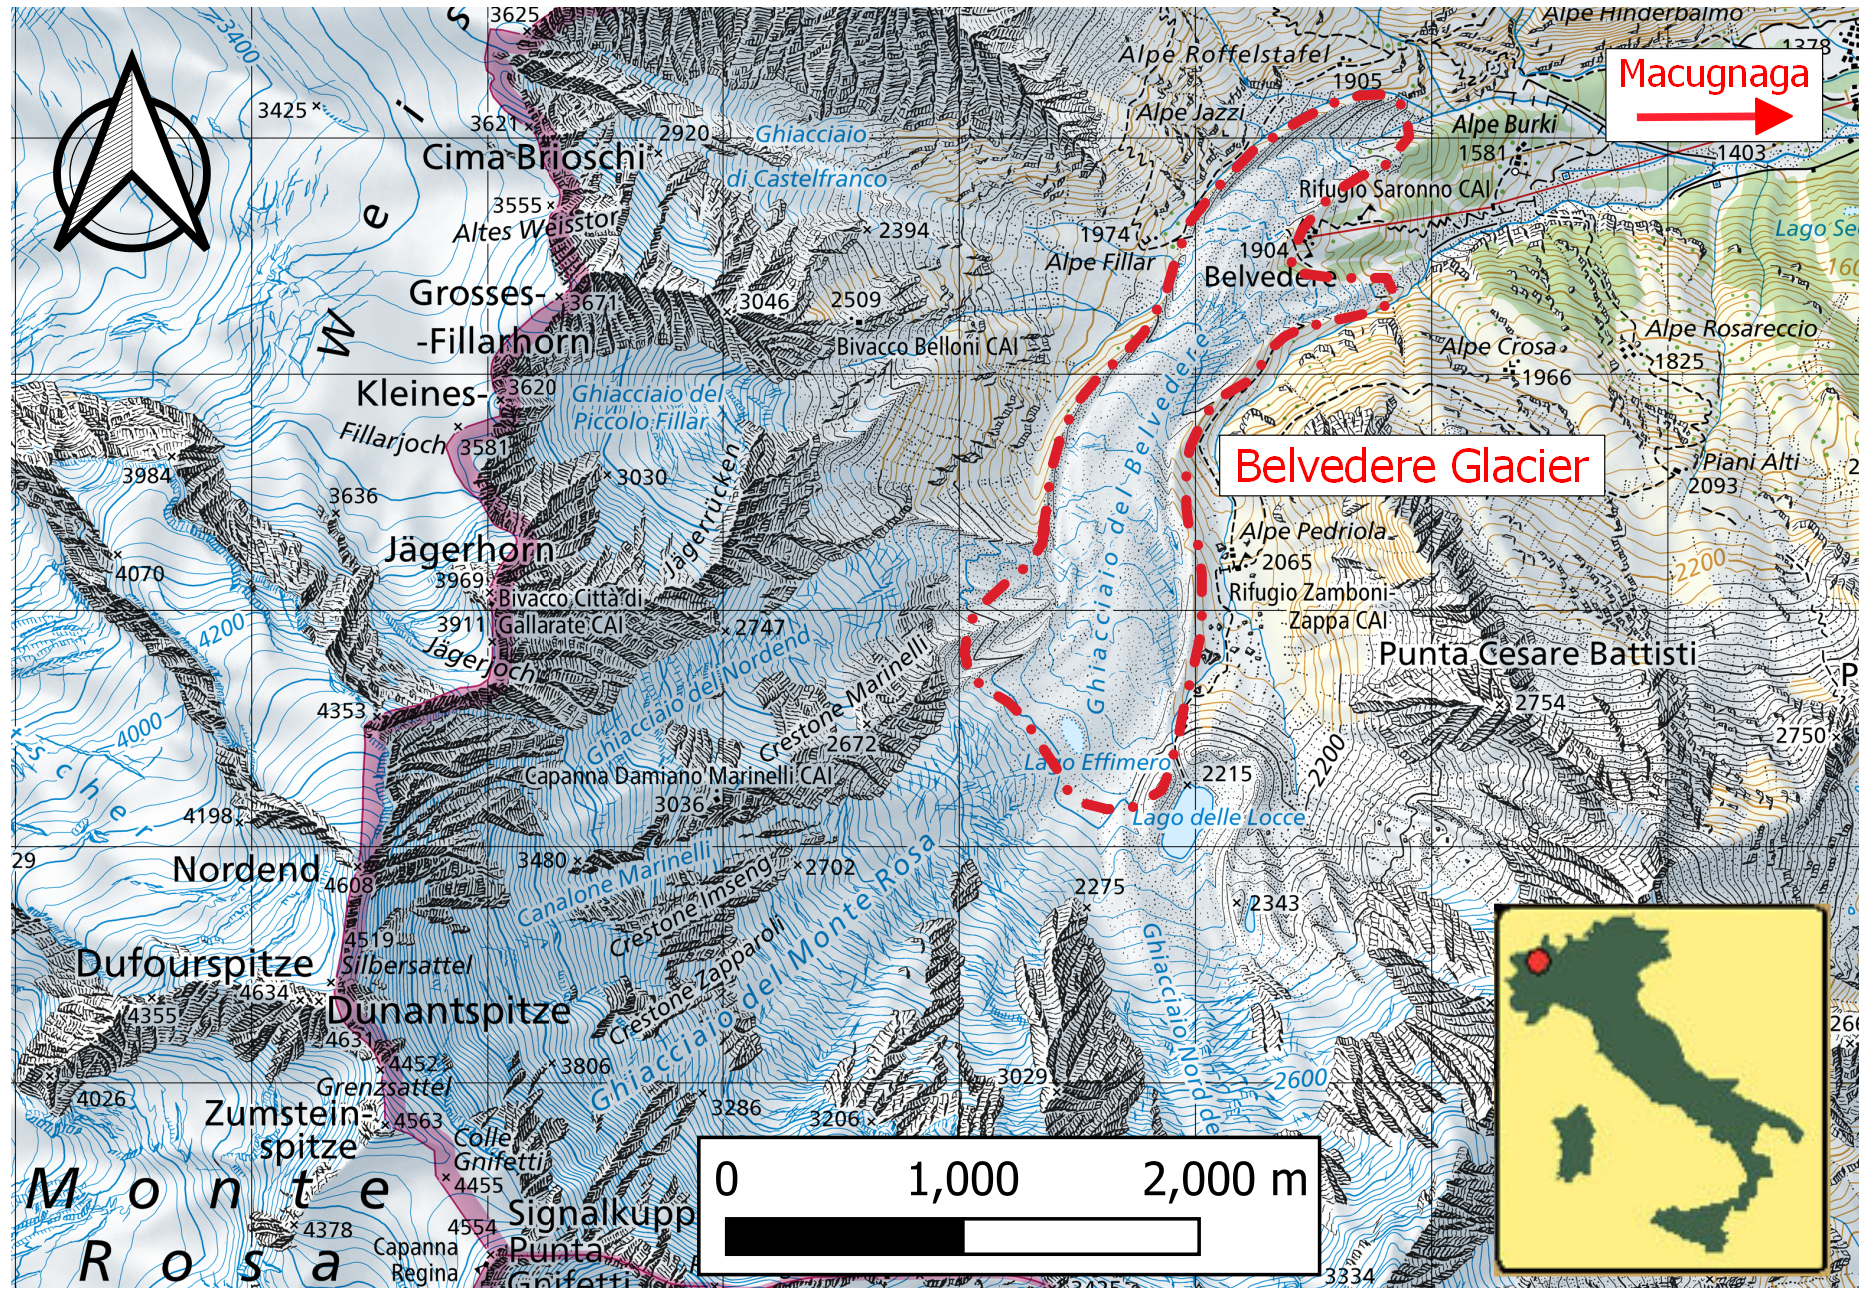
\includegraphics[height=5cm]{belvedere_location.png}
    }
    \subcaptionbox{\label{fig:1:studyarea:pic}}{
        \includegraphics[height=5cm]{belvedere_pic.jpg}
    }
    \caption{(a) Location of Belvedere Glacier, base map (source: Swisstopo
        www.geo.admin.ch); (b) Picture of the Belvedere Glacier taken from the nearby Monte Moro.}
    \label{fig:1:studyarea}
\end{figure}

In the past, several hazardous events originated from the Belvedere Glacier, such as floods
and slope instability, threatened the nearby village of Macugnaga and the Zamboni Zappa
Hut, at 2070 m a.s.l. \citep{Kaab2004}.
At the beginning of the 21st century, the Belvedere Glacier was characterized by a
particular surge-type dynamics  \citep{Haeberli2002}.
During the late 1990s, the~surface speeds of the whole glacier were ranging between
\SIlist{30;45}{\meter\per\year}~\citep{Roethlisberger1985, Kaab2005}.
During 2000--2001 an accelerated flow in the Monte-Rosa Glacier produced a wave of
compression-decompression stresses and strains in the Belvedere Glacier.
Surface velocities soared: values up to \SI{200}{\meter\per\year} were observed
photogrammetrically during autumn 2001~\citep{Kaab2004}.
The ice thickness increased more than~\SI{20}{\meter} and the wave travelled downwards,
creating a depression area in the accumulation zone, that was filled by a super-glacial
lake, the Lago Effimero~\citep{Haeberli2002, Mortara2009}.

During spring 2002, the large depression at the foot of the Monte Rosa east face, caused by the 
surge-type movement was temporarily filled by a lake with a volume of \SI{3e6}{\cubic\meter}, 
the socalled \textit{Lago Effimero} (\textit{short-lived lake}).
Recognizing the potential danger of an outburst flood, the Italian Civil Defense Department rapidly 
implemented emergency measures, including evacuating parts of Macugnaga village, installing automatic 
alarm systems and pumps, and initiating detailed scientific investigations. 
Reduced meltwater input in July 2002, combined with natural subglacial drainage, stabilized and subsequently 
lowered the lake level.
However, the lake reformed in the spring of 2003 and it burst out in mid-June of that year without causing 
any significant damage \citep{Kaab2004}.

\textcolor{red}{Expand this part and add more pics with old and recent events}

% The northern lobe of the Belvedere Glacier is concurrently experiencing a fast retreat:
% in the past few years, an average retreat of \SI{\sim20}{\meter\per\year} was documented
% \citep{Ioli2022} and it is actively changing every day, due to ice falls and collapses.

\section{Thesis outline}

% References
\makechapterbibliography{}
\graphicspath{{figures/chapter2/}}

\chapter{Back to the past: reconstructing glacier geometry with historical aerial images
  (1977-2009)}\label{ch:2}

\vfill

\newthought{This chapter is based on:}

\noindent De Gaetani, C. I., Ioli, F., \& Pinto, L. (2021). Aerial and UAV Images for
Photogrammetric Analysis of Belvedere Glacier Evolution in the Period 1977–2019. Remote
Sensing, 13(18), 3787. \url{https://doi.org/10.3390/rs13183787}

\newpage

\section{Introduction}\label{sec:2:introduction}

\section{Datasets}\label{sec:2:datasets}

\subsection{Historical Aerial Datasets of 1977, 1991 and 2001}

\subsection{Digital Aerial and UAV Datasets of 2009 and 2019}

\subsection{GNSS Survey for Block Georeferencing}

\section{Methods}\label{sec:2:methods}

\section{Discussion}\label{sec:2:discussion}

% References
% \bibliography{references}
% \addcontentsline{toc}{section}{References}
% \bibliographystyle{apacite}

\graphicspath{{figures/chapter3/}}
\onehalfspacing

\chapter{UAV photogrammetry for annual glacier reconstruction (2015-2023)}\label{ch:3}

\vfill

\newthought{This chapter is based on:}

\noindent Ioli, F., Bianchi, A., Cina, A., De Michele, C., Maschio, P., Passoni, D., \&
Pinto, L. (2021). Mid-Term Monitoring of Glacier’s Variations with UAVs: The Example of
the Belvedere Glacier. Remote Sensing, 14(1), 28.
\url{https://doi.org/10.3390/rs14010028}

\newpage

{\color{red} TODO: move the definition of the three sectors in discussion (experimentally bases!). Remove all references to sectors before that.}


\section{Introduction}\label{sec:3:intro}

{\color{red} TODO}


\section{Instruments and datasets}\label{sec:3:instrument}

{\color{red} Short intro to section...}

 
\subsection{GNSS measurements}\label{sec:3:gnss}

A set of GCPs was materialized with square cross targets, printed on polypropylene sheets
and anchored on big rocks (\figref{fig:3:belvedereGCP}b).
About 25 targets were deployed over the glacier (named hereafter as \textit{moving targets} or \textit{M\#} in \figref{fig:3:belvedereGCP}a) and 24 targets (labelled as 
\textit{stable targets} or \textit{S\#} in \figref{fig:3:belvedereGCP}a) were placed on
stable areas along the moraines so that they were not subjected neither to the ice flow
nor to rock falls.
Every year, the condition of each target was checked and, if one was damaged or
destroyed, the polypropylene sheet was replaced by keeping the same location of the
center (i.e., by using the same fisher plugs).
During the years, some targets were lost, and therefore new ones were materialized (e.g.,
M29bis).
Targets were yearly surveyed with dual frequency (L1/L2) geodetic quality GNSS receivers
and their coordinates were framed within the official Italian reference system ETRF2000
at the epoch 2008.0, projected in UTM 32N.
For the lower part of the glacier, where the GSM network connection was available, target
position was obtained in nRTK with respect to a network of CORS permanent stations
(either HxGN SmartNet or SPIN GNSS).
The points were occupied at least twice, each time for a duration of \qty{5}{\second}.
By contrast, in the upper part of the glacier, targets were surveyed with static sessions
of \qty{\sim 10}{\minute}, and raw observation data was post-processed with respect to
local master stations, located on stable and well known points.
To this end, either the point \textit{S12}, placed on a big rock next to the
Zamboni-Zappa hut, or the point \textit{S20}, located near the Rifugio Ghiacciai del Rosa
on the Belvedere hill,	were used (see \figref{fig:3:belvedereGCP}a).
Accuracy of GNSS measurements was evaluated empirically by comparing repeated
measurements over stable targets carried out in different years.
RMSE of \qty{1.5}{\centi\meter} in planimetry and \qty{3}{\centi\meter} in elevation were
obtained.

\begin{figure}
    \centering
    \subcaptionbox{\label{fig:3:3:studyarea:map}}{
        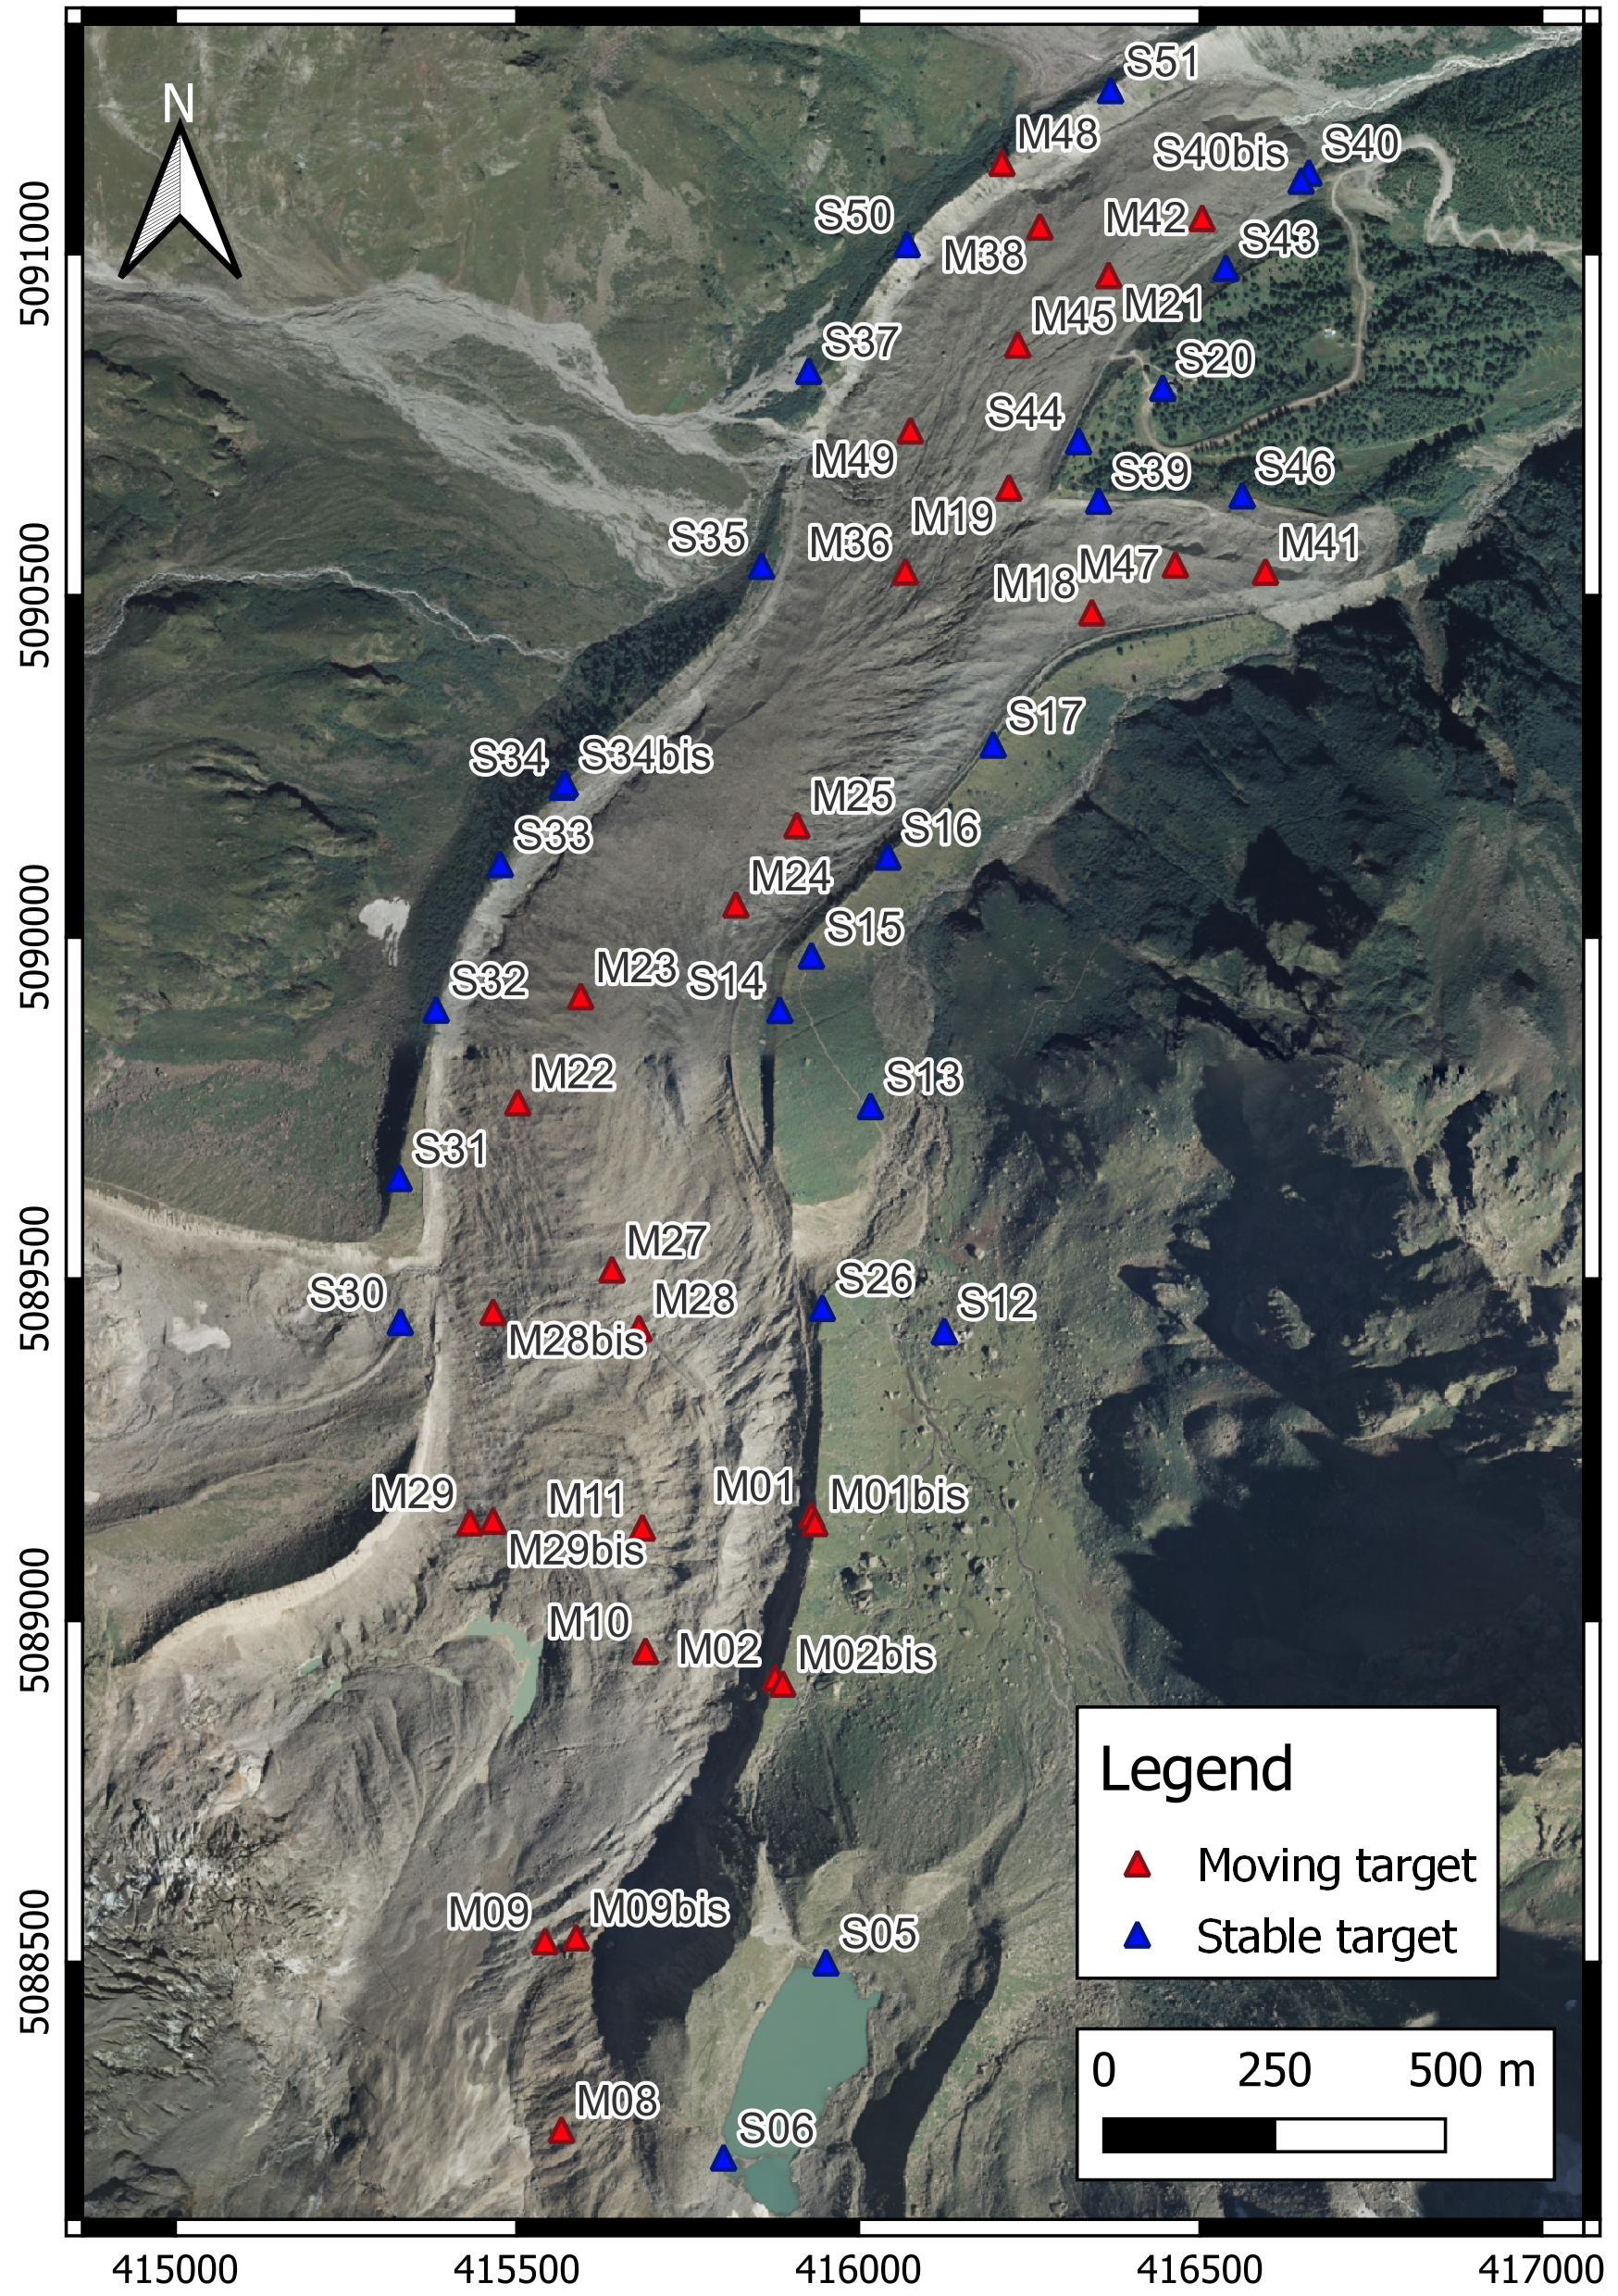
\includegraphics[width=.6\textwidth]{belvedereGCP.png}
    }
    \subcaptionbox{\label{fig:3:3:studyarea:pic}}{
        \includegraphics[width=.35\textwidth]{target.jpg}
    }
    \caption{(\textbf{a}) An example of a photogrammetric target deployed over the
        glacier moraine; (\textbf{b}) location of the targets used for the
        photogrammetric
        surveys. For~each year, a~subset of the targets were used as GCPs, while the
        remaining
        as~CPs.}
    \label{fig:3:belvedereGCP}
\end{figure}


\subsection{UAV flights}\label{sec:3:uav-flights}

Because of the long duration of the monitoring campaign, the challenging environment and
the fact that more than one research group was involved in the project, different UAV
platforms and cameras were used.
As reported in \tabref{tab:3:datasets}, in~2015 and 2016, a~ready-to-fly fixed-wing UAV
SenseFly eBee, equipped with a compact camera Canon PowerShot S110, was employed to
survey the whole glacier.
During 2017, different combinations of UAVs (fixed-wing and quadcopters) and cameras were
employed (\tabref{tab:3:datasets}).
From 2018 to 2020, a~low-cost recreational fixed-wing UAV Parrot Disco FPV, with~a
wingspan of \SI{1.15}{\meter} and a weight of \SI{750}{\gram}, was adapted to carry a
small and lightweight action cam Hawkeye Firefly~8S.
For each camera, the main sensor and objective characteristics are listed
\tabref{tab:3:camere}.

UAVs flights were conducted automatically by using ground station software packages
developed by UAV manufacturers.
    {\color{red} Add UGCS...}

The flights were designed to have GSD ranging between \qtylist{5;10}{\centi\meter}, and
to guarantee \qty{\sim 80}{\percent} of longitudinal and \qty{\sim 60}{\percent} of
transversal overlap.
Average image GSD values and number of GCPs and CPs, used respectively to orient the
images and to assess the quality of the photogrammetric blocks, are summarized in
\tabref{tab:3:datasets}.

{\color{red} Add instruments for 2021-2023...}

\begin{table}[p]
    \small
    \centering
    \caption{Summary of the characteristics of the surveys.}
    \begin{tabular}{c  m{1.8cm} m{3.5cm} m{4.2cm} c c c }
        \toprule
        Year                                                              & Date
                                                                          & UAV
                                                                          & Camera
                                                                          & GSD
                                                                          & GCP
                                                                          & CP
        \\
                                                                          &
                                                                          &
                                                                          &
                                                                          & [m/px]
                                                                          & [\#]
                                                                          & [\#]
        \\
        \midrule
        2015                                                              & A.
        8.10\newline B. 23.10                                             &
        SenseFly eBee                                                     & Canon
        PowerShot S110                                                    & 0.07
                                                                          & 24
                                                                          & 11
        \\[4mm]
        2016                                                              & 20.10
                                                                          & SenseFly eBee
                                                                          & Canon
        PowerShot S110                                                    & 0.09
                                                                          & 31
                                                                          &
        15
        \\[4mm]
        2017                                                              & A.
        5.10\newline B. 15.11\newline C. 16.11                            & A. SenseFly
        eBee \newline B. SenseFly eBee Plus\newline  C. DJI Phantom 4 Pro & A. Canon
        PowerShot
        S110  \newline B. SenseFly S.O.D.A \newline C. DJI FC6310         & 0.06
                                                                          & 27
                                                                          & 8
        \\[4mm]
        2018                                                              & 23-25.07
                                                                          & Parrot Disco
                                                                          & Hawkeye
        Firefly 8S                                                        & 0.05
                                                                          & 27
                                                                          &
        13
        \\[4mm]
        2019                                                              & 29.07-2.08
                                                                          & Parrot Disco
                                                                          & Hawkeye
        Firefly 8S                                                        & 0.06
                                                                          & 26
                                                                          &
        10
        \\[4mm]
        2020                                                              & A. 26-27.07
        \newline B. 9.08                                                  & A.
        Parrot Disco\newline B. DJI Phantom 4 Pro                         & A. Hawkeye
        Firefly 8S\newline B. DJI FC6310                                  &
        0.05                                                              & 29
                                                                          & 12
        \\[4mm]
        2021                                                              & 29.07-2.08
                                                                          & DJI Matrice 210 V2
                                                                          & DJI ZenMuse x5s
                                                                          & 0.04
                                                                          & 23
                                                                          &
        9
        \\[4mm]        
        2022                                                              & 28.07-29.07
                                                                          & DJI Matrice 300 RTK
                                                                          & DJI Zenmuse P1 - 35 mm
                                                                          & 0.03
                                                                          & 22
                                                                          &
        19
        \\[4mm]
        2023                                                              & 25.07-27.07
                                                                          & DJI Matrice 300 RTK
                                                                          & DJI Zenmuse P1 - 35 mm
                                                                          & 0.03
                                                                          & XX
                                                                          &
        XX
        \\[4mm]        
        \bottomrule

    \end{tabular}
    \label{tab:3:datasets}
\end{table}

\begin{table}[p]
    \centering
    \small
    \caption{Summary of the characteristics of the cameras employed.}
    \begin{tabular}{c c c c c c}
        \toprule
        Camera                        & Sensor                        & Sensor Size
                                      & Focal length                  & Image size
                                      & Pixel size
        \\
                                      &                               &
        [\SI{}{\milli\meter\squared}] & \newline[\SI{}{\milli\meter}] & [\SI{}{\pixel}]
                                      & \newline[\SI{}{\micro\meter}]
        \\

        \midrule
        Canon PowerShot S110          & 1/1.7" CMOS                   & $7.44\times5.58$
                                      & 5.2                           & $ 4000 \times
            3000
        $                             & 1.9
        \\
        SenseFly S.O.D.A              & 1" CCD                        & $13.2\times8.8$
                                      & 10.6                          & $5472 \times
        3648$                         & 2.4
        \\
        DJI FC6310                    & 1" CMOS                       & $13.2\times8.8$
                                      & 8.8                           & $5472 \times3648$
                                      & 2.4
        \\
        Hawkeye Firefly 8S            & 1/2.3" CMOS                   & $6.17\times4.56$
                                      & 3.8                           & $5472 \times3648$
                                      &
        1.34
        \\
        DJI ZenMuse x5s               & 4/3" CMOS                     & $17.3\times13$
                                      & 15                            & $5280 \times
        3956$                         & 3.3 
        \\
        DJI Zenmuse P1 - 35 mm        & FullFrame CMOS                & $35.9\times24$
                                      & 35                            & $8192 \times
        5460$                         & 4.4
        \\
        \bottomrule
    \end{tabular}
    \label{tab:3:camere}
\end{table}

\subsection{Problems Arisen during the surveys of 2017 and~2020 {\color{red} REVISE}} \label{sec:3:problems} 
% Compared to traditional glaciological techniques, UAVs allow for a significant reduction of in-situ operations (limited to surveying few GCPs spread along the glacier and performing UAV flights).
Conducting a yearly monitoring campaign in an alpine environment for~six consecutive
years is challenging because of, for example,~the hard accessibility of some areas of the
glacier (also for fixed-wing UAVs take-off and landing) and the variability of the
meteorological~conditions.

Adverse meteorological conditions and practical issues made it necessary to split the
2017 survey in different dates, and~various UAVs and cameras were employed (see
\tabref{tab:3:datasets}).
The 2017 photogrammetric model was therefore divided into three parts: the central part
refers to the October survey while the lower and the upper parts refer to the November
survey and at that time the glacier was covered by snow (\figref{fig:3:ortophoto}c).
Technical problems arose also during the 2020 survey: a breakage of one elevon servo
during a landing phase caused the fixed-wing UAV to crash.
Therefore, a~quadcopter DJI Phantom 4 Pro was employed to survey the upper part of the
glacier (approximately the S1 sector, see the different colors in the orthophoto of
\figref{fig:3:ortophoto}f) 14 days after the former.
However, during~the August 2020 fieldwork, it was not possible to measure any additional
GCPs because the south-west part of the Belvedere Glacier, close to the Monte-Rosa
Glacier is hardly accessible and dangerous due to the presence of crevasses and steep
rocks.
The few GCPs available in the upper part of the glacier made necessary to co-register the
Phantom 4 Pro model on the 2019 model, by~searching for sharp edges of rocks along the
moraines, remained fixed along the year, on~ 2019 images.
This approach is less accurate than measuring targets directly on the field.
The RMSE on CPs was therefore equal to \SI{0.36}{\meter} (see
\figref{fig:3:CP_errors}), \SI{\sim 7}{}~times the GSD.
Nevertheless, the~area affected by this issue was rather limited, compared to the whole
Belvedere~Glacier.

Moreover, between~2017 and 2018, the~survey period was moved from Autumn to Summer.
From 2015 to 2017, in~fact, field works were included within the DREAM project (see
\secref{sec:3:intro}) and they took place in Autumn, at~the beginning of the academic
year.
By contrast, from~2018 to 2020, surveys were carried out at the end of July because they
were encompassed within a Summer School organized by DICA (Politecnico di Milano).
The change in the survey dates was critical because the timespan occurred between the
survey of October/November 2017 and that of July 2018 did not include the period of
maximum ablation and velocity of the glacier (neither August 2017 nor August 2018).
Therefore, volume variation and ice flow velocity refer mostly the wintertime and the
results obtained are not directly comparable with those of the other~years.


\section{Metodology}\label{sec:3:methodology}

\subsection{SfM workflow}\label{sec:3:sfm}

In order to build photogrammetric models of the glacier, images acquired during UAV
surveys were processed with the SfM software Agisoft Metashape 1.7.2 \citep{agisoft}.
For each year, at least 24 GCPs spread over the glacier were employed to orient the
images, whereas at least 10 Check Points (CPs) were used to assess models quality.
Both GCPs and CPs were manually collimated on the images.
Tie Points (TPs) were detected and matched by Metashape on full resolution images (which
corresponds to \textit{high accuracy} parameter in Metashape).
Image External Orientation (EO) and TPs world coordinates were estimated by solving the
Bundle Block Adjustment (BBA).
TPs with the worst reprojection error on images, which are likely originated from false
matches, were removed and the BBA was solved again to improve quality of BBA solution.
This process was iterated more times until TPs mean reprojection error had dropped below
\SI{\sim 0.8}{\pixel}.
Camera internal orientation was estimated by self-calibration
\citep{Fraser2013,Cramer2017}, because of its instability in the cameras employed.

Dense 3D reconstruction was computed by Agisoft Metashape with proprietary MVS
algorithms~\citep{Dallasta}.
Depth maps and dense point clouds were obtained from images downsampled by a factor 4,
in~order to reduce the computational time (\textit{medium quality} parameter of the dense
cloud generation in Metashape).
Triangulated mesh surfaces and photorealistic textures were~computed.

DSMs with a resolution of \SI{0.5}{\meter\per\pixel} were derived from the mesh model.
Finally, orthophotos with a GSD of \SI{0.10}{\meter\per\pixel} were obtained by
projecting the most nadiral images over the mesh model (\figref{fig:3:ortophoto}).

\subsection{Glacier flow velocity}\label{sec:3:method_velocity}

{\color{red} TODO}

In case of debris-covered glacier, big rocks and boulders usually move jointly with the ice flow \textcolor{red}{REF}, 
Therefore, it was possible to investigate ice flow dynamics and to estimate glacier surface velocity by evaluating debris pattern movements.
In-situ GNSS measurements of the \textit{moving targets}, deployed over big rocks (see~\secref{sec:3:gnss}),  were first employed to estimate yearly average velocities of the glacier.
Targets coordinates, measured on different years, were differentiated and the annual average velocity of each point was derived by dividing the displacement by the time lag. 
These punctual velocity measurements are hereafter labelled as \textit{GNSS} and they can be considered as high accurate (i.e., centimetric) measurements of glacier displacements and velocities.

{\color{red} ADD DIC}

The number of GNSS measurements are limited to a dozen of points spread over the glacier, consequently they are not enough to derive a complete glacier velocity field.
Hence, DIC algorithms, such as normalized cross-correlation or orientation correlation~\citep{Heid2012_evaluation_xcorr} are widely applied to automatically compute displacement on orthophotos and might allow for sub-pixel accuracy \citep{Debella_Gilo2011}.	

{\color{red} motivate MAN because of snow and validation of DIC}

Additionally, a set of features were manually collimated on orthophotos and tracked over the years to obtain complete surface velocity fields.
These points are named as \textit{MAN}.

However, because of the presence of snow and due to significantly different environmental conditions between years (\figref{fig:3:ortophoto}), it was not feasible to apply automatic image matching algorithms on all the orthophotos to obtain displacements between corresponding pattern of pixels. 
Therefore, the visual collimation of characteristic features (e.g., sharp edges of big rocks emerging from the snow) on different orthophotos was the only possibility to track elements on the glacier surface. 
Even though manual collimation precision of natural elements, such as rocks, on orthophotos was likely worse compared to computer vision algorithms, a human operator supervision ensured high matching reliability.
Moreover, it was possible to define a regular grid of \qtyproduct{100 x 100}{\metre} on the orthophotos in order to select homogeneously distributed features (\qty{\sim 1}{\pt} every \qty{10000}{\meter\squared}), resulting in a total of \qty{\sim 130}{points}.
Most of the points were tracked over the years; however some were lost and only \qty{115}{points} were found on the 2020 orthophoto.


\subsection{Volume variations}\label{sec:3:method_volumes}

To compute glacier volume variation $ \Delta V $, consecutive DSMs were differentiated
by~employing a DEM of Difference (DOD) approach with the tool \textit{Compute 2.5D volume} implemented in CloudCompare~\citep{cloudcompare}.
First, photogrammetric dense clouds were gridded by projecting points along the vertical
direction on a planar surface, obtaining DSMs with a cell footprint on ground of \qtyproduct{0.5x0.5}{\meter}.
The choice of the raster resolution was a compromise to achieve a robust height field
estimation by averaging a large enough number of points for each cell of the raster,
but~at the same time small enough to maintain a spatial resolution able to map small
scale glacier morphology.
A mask was manually created and applied to all the DSMs to exclude areas outside the
glacier surface.
DSMs from consecutive years were then differentiated pixel-by-pixel to obtain the height
difference at each cell of the raster.

In order to rigorously estimate volume variation variances, by~propagating the variance,
it would be  necessary to know the covariance matrix of each DSM, considered as a
multivariate random variable with dimension equal to the number of cells.
However, no information concerning cells covariances was provided by the SfM software
employed, thus it was troublesome to compute covariances between nearby cells in a DSM
(which are clearly correlated because they were generated by the same set of images in
the photogrammetric process).
As a consequence, only a rough estimation of the variance was carried out by considering
each DSM as a mono-dimensional random variable with variance equal to the squared value
of the vertical component of RMSE computed on the CPs of the relative photogrammetric
model.
Moreover, $ DSM^{(i+1)} $ and $ DSM^{(i)} $ were considered as independent because there
was no relation between the surveys.
The variance of the volume variation was therefore computed as:
\begin{equation}
    \sigma^2_{\Delta V^{(i+1,i)}}  = {(n \times A_c)}^2 \left( \sigma^2
    _{DSM^{(i+1)}} + \sigma^2_{DSM^{(i)}} \right),
    \label{eq:3:volVarProp}
\end{equation}
where $ n $ is the number of cell in the~DSMs and $ \sigma^2 _{DSM}$ is the squared
vertical error of the photogrammetric model evaluated on the GCPs.

For the years 2015--2016, 2016--2017, 2017--2018, the~glacier was partially covered by
snow (see \figref{fig:3:ortophoto}a--c), which introduced additional uncertainties in
volume estimation.
The snow height accumulated at the nivometric station located near Zamboni Zappa Hut
(2075 m a.s.l., in~the central sector of the glacier) on the survey dates was retrieved
from the meteorological database of ARPA Piemonte, the~regional agency for the
environment~\citep{arpaPie}: \SI{22}{\centi\meter} of snow were measured on 23 October
2015, \SI{20}{\centi\meter} on 20 October 2016, \SI{40}{\centi\meter} on 15 November 2017.
The measured snow heights were considered as additional components of DSM standard
deviations.
Yet, because~the glacier was only partially covered by snow, the~snow-driven uncertainty
was weighted by half of the total glacier area in variance propagation.

\subsection{Glacier outline}\label{sec:3:method_outline}

{\color{red} TODO}

\section{Results}\label{sec:3:res}

\subsection{SfM}\label{sec:3:res:sfm}

\begin{figure}
    \centering
    \includegraphics[width=0.7\columnwidth]{CPrmse.png}
    \caption{Barplot of reprojection RMSE computed CPs for each photogrammetric
        model. Due to practical problems occurred in 2020 and explained in
        \secref{sec:3:problems}, the~RMSE of 2020 model was split in two parts:
        \textit{2020 lower} denotes the CP RMSE over related to the central and 
        lower sectors of the glacier (S2 and S3 in \figref{fig:3:belvedere}a), 
        whereas \textit{2020 upper} refers to the upper accumulation sector 
        only (S1). {\color{red} remove 2020 upper and add recent years}}
    \label{fig:3:CP_errors}
\end{figure}

\begin{figure}
    \centering
    \subcaptionbox{\label{fig:3:ortophoto:2015}}{
        \includegraphics[width=0.30\textwidth]{orto2015.jpg}
    }
    \subcaptionbox{\label{fig:3:ortophoto:2016}}{
        \includegraphics[width=0.30\textwidth]{orto2016.jpg}
    }
    \subcaptionbox{\label{fig:3:ortophoto:2017}}{
        \includegraphics[width=0.30\textwidth]{orto2017.jpg}
    }
    \\
    \subcaptionbox{\label{fig:3:ortophoto:2018}}{
        \includegraphics[width=0.30\textwidth]{orto2018.jpg}
    }
    \subcaptionbox{\label{fig:3:ortophoto:2019}}{
        \includegraphics[width=0.30\textwidth]{orto2019.jpg}
    }
    \subcaptionbox{\label{fig:3:ortophoto:2020}}{
        \includegraphics[width=0.30\textwidth]{orto2020.jpg}
    }
    \subcaptionbox{\label{fig:3:ortophoto:2021}}{
        \includegraphics[width=0.30\textwidth]{orto2020.jpg}
    }
    \subcaptionbox{\label{fig:3:ortophoto:2022}}{
        \includegraphics[width=0.30\textwidth]{orto2020.jpg}
    }
    \subcaptionbox{\label{fig:3:ortophoto:2023}}{
        \includegraphics[width=0.30\textwidth]{orto2020.jpg}
    }
    \caption{Orthophotos obtained from the photogrammetric model for each year.
        (\textbf{a}) 2015, (\textbf{b}) 2016, (\textbf{c}) 2017, (\textbf{d}) 2018,
        (\textbf{e})
        2019, (\textbf{f}) 2020, (\textbf{g}) 2021, (\textbf{h}) 2022, (\textbf{i})
        2023. {\color{red} Add recent years}}
    \label{fig:3:ortophoto}
\end{figure}

The re-projection RMSE over the CPs are shown in \figref{fig:3:CP_errors} as assessment
of the geometrical accuracy of the models.
The global re-projection RMSE was mostly ranging between \SIlist{0.1;0.2}{\meter}.
The only exception consisted in the {\color{red} upper sector (comparable to sector S1 in
\figref{fig:3:belvedere}a) of the 2020 model}, for~which the RMSE is almost double
compared to the other values.
{\color{red}
This was caused by practical problems occurred in 2020, explained in detail in
\secref{sec:3:problems}.
}
As a consequence, the~value of 2020 RMSE was split in two different bars in the graph.
From 2015 to 2017, when compact cameras were used, errors comparable to 1.5 times the GSD
were obtained.
Since 2018, a~lightweight action-cam has been employed to minimize the UAV take-off
weight and this has led to an RMSE up to 3~times the GSD, but~still always smaller than
\SI{0.2}{\meter}.

\subsection{Glacier flow velocity}\label{sec:3:res:velocity}
{\color{red} TODO}

Annual ice flow velocities were first computed from in-situ GNSS measurements of \textit{moving targets}.
\figref{fig:3:GNSS_velocity} shows the time-series of the velocities of GNSS points. 
Most of the moving targets were found and measured for 3 or more years and some of them have been continuously tracked since 2015 (e.g., the point \textit{M10} in the upper part of the glacier, \textit{M28} in the middle part or \textit{M41} on the south-east tongue). 
However, some of them have been lost over the year, e.g. because they fell into a crevasse, and they were replaced with new ones. 
The location accuracy of the GNSS measurement was estimated as \qty{\sim 3}{\centi\meter} (see Section~\ref{sec:3:gnss}). 
Assuming measurements of the same GCPs at two consecutive years as independent,
the expected standard deviation of the velocity was computed by propagating the variance as \qty{\pm 0.04}{\meter\per\year} (i.e., two order of magnitude less than the computed annual velocities which ranges between \qtylist{2;22}{\meter\per\year}).
Therefore, GNSS measurement are considered as the reference source of information for flow velocity estimation.

From graph in \figref{fig:3:GNSS_velocity}, GNSS points can be visually grouped in three clusters (C1, C2, C3) on the basis of velocity magnitude. 
The first low-velocity cluster C1 includes points with velocities between  \qtylist{2;7}{\meter\per\year}. 
{\color{red}
The location of GNSS points included in C1 well match morphological sectors S1 (upper accumulation sector) and S3 (glacier tongues), marked in \figref{fig:belvedere}a.
By contrast, cluster C3 presents significantly higher speed, ranging between \qtylist{17;22}{\meter\per\year} were sensed in the central sector S2 (e.g., \textit{M10, M11, M22, M28}).
Cluster C2 include GNSS points located in transition areas between S2 and S1 (e.g., targets \textit{M10, M11}, placed between the central sector and the accumulation area) and between S2 and S3 (e.g., \textit{M49}, between the central sector and the lower north-west tongue).
}

{\color{red} Move to discussion: 
Measurements of targets \textit{M22, M23} and \textit{M28} suggests the presence of a rising velocity trend in the central part of the glacier between 2018 and 2020. 
In fact, these points experienced an increase of the velocity magnitude of \qty{\sim 1}{\meter\per\year} from 2018 to 2020.
However, some more measurement years would be necessary to state if this increasing velocity trend holds and is significant. 
On the other hand, all the other targets showed rather steady velocities over the 6 years.
}

\begin{figure}
    \subcaptionbox{\label{fig:3:GNSS_velocity:ts}}{
        \includegraphics[width=0.68\textwidth]{GCPghiacciaioSerieTemp_02}
    }
    \subcaptionbox{\label{fig:3:GNSS_velocity:map}}{
        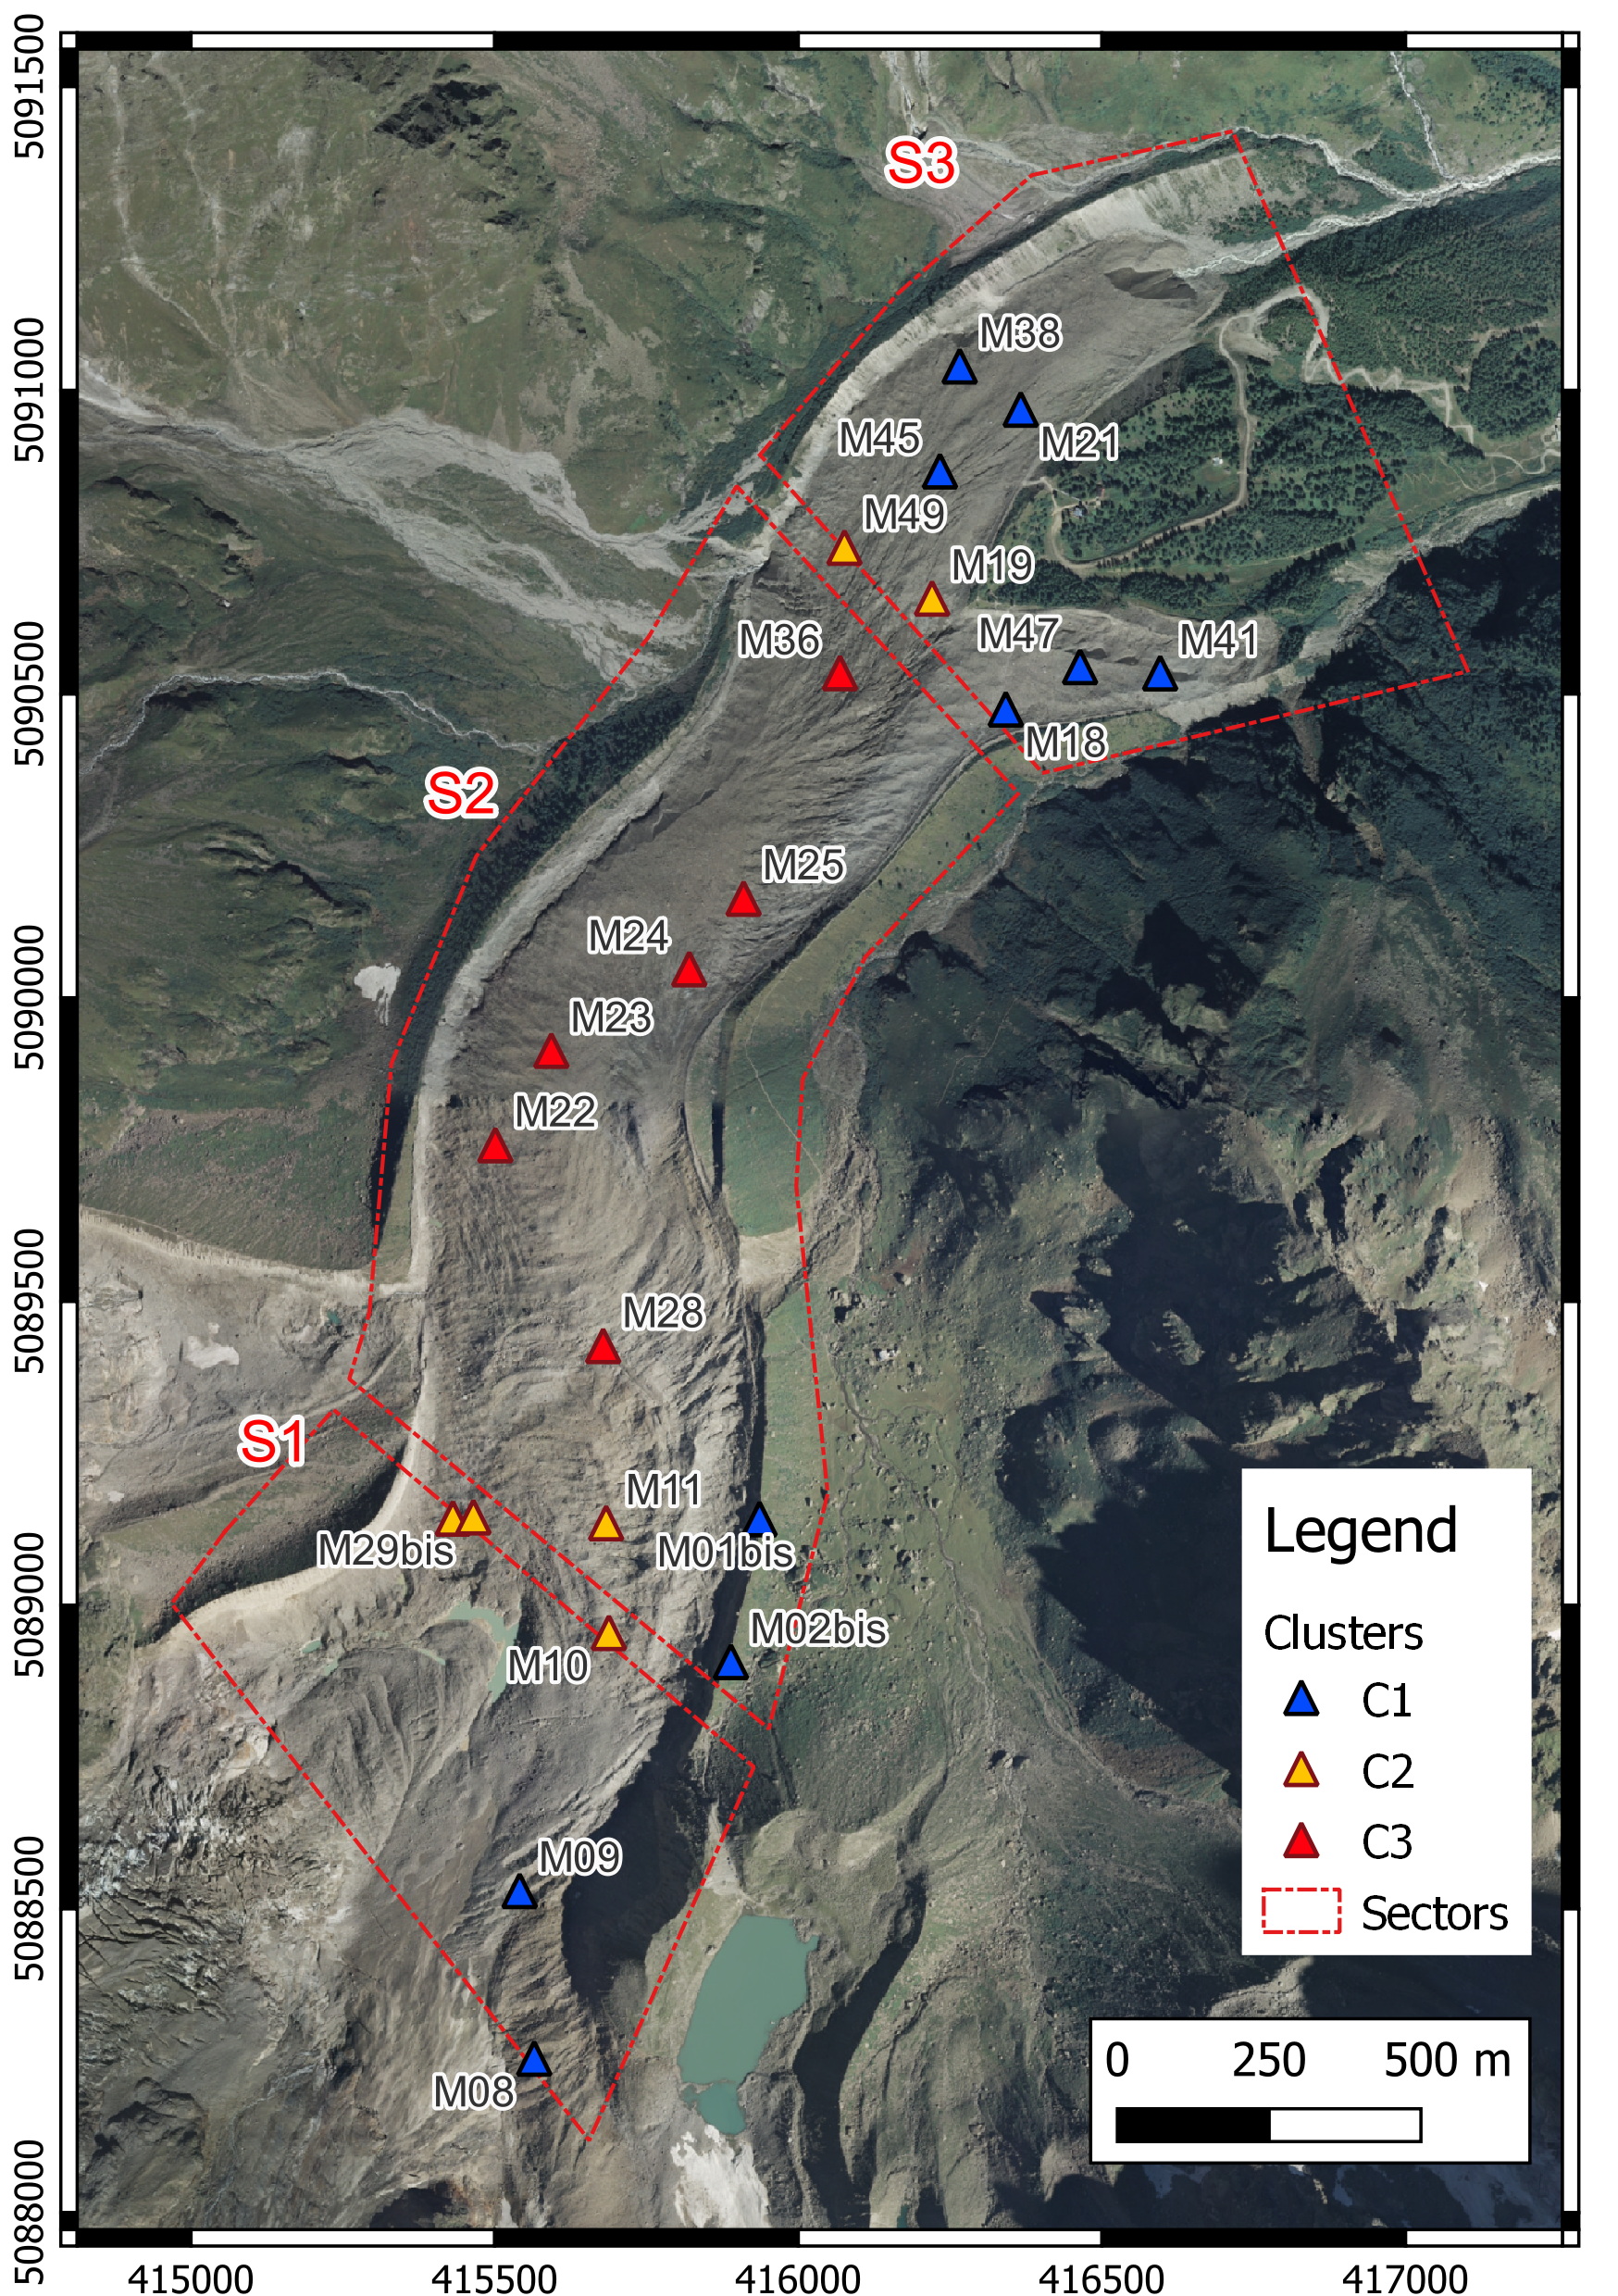
\includegraphics[width=0.29\textwidth]{GCPghiaccaio_clusters}
    }
    \caption{\textbf{(a)} Time series of the velocity computed from the GNSS measurements of the targets deployed over the glacier. Dashed lines denote measurement continuity over the years (i.e., if the line is interrupted, the target was lost or not measured during that year). Labels C1-C3 denote the three velocity clusters of GNSS points, whereas labels S1-S3 indicate the three morphological sectors marked in \figref{fig:belvedere}a. A correspondence between clusters and sectors can be identified: C1 corresponds to sectors S1 and S2, cluster C3 to sector S2, whereas cluster C2 corresponds to the two transition areas S2-S1 and S2-S3. \textbf{(b)} Location of the targets over the glacier.}
    \label{fig:3:GNSS_velocity}		
\end{figure}

\subsection{Volume variations}\label{sec:3:res:volumes}

{\color{red} Add 2021-2023!}

\begin{figure}
    \centering
    \includegraphics[width=0.8\columnwidth]{volume_loss_2015-2023.png}
    \caption{Yearly volume variation computed as difference between DSM of two
        consecutive years. The~error bars plotted represent the uncertainty of each
        estimated value. Note that the values on the Y axis are expressed in million of
        \si{\cubic\meter}.}
    \label{fig:3:volumes}
\end{figure}

\figref{fig:3:volumes} illustrates the loss of ice volume year by year.
The estimated variance of the glacier volume variation is plotted as an error bar for
each value of volume~variation.

Between 2017 and 2018, field works were moved from Autumn to Summer.
Therefore, the~loss of volume for the year 2017--2018 was computed between October 2017
and July 2018, therefore it represented only the variation occurred in wintertime and
springtime, and~it should not be directly compared with the annual average.
Indeed, 2017--2018 volume variation was \SI{-0.75e6}{\cubic\meter}, against~the average
variation between 2015 and 2020 of \SI{-2.81e6}{\cubic\meter} (difference of
\SI{27}{\percent}).
Ice volume loss for the year 2019--2020 may be slightly underestimated as well: the
photogrammetric model of the upper part of the glacier was affected by a larger geometric
(RMSE in vertical direction of \SI{0.28}{\meter}, see \secref{sec:3:problems})
compared to the others models, due to the lack of GCPs measured in-situ at the time of
the photo acquisition.
Overall, the~negative ice volume variation occurred between 2015 and 2020 is evident and
significant: every year, between~\SIlist{2e6;3.5e6}{\cubic\meter} of ice were~lost.

\begin{figure}
  \centering
  \subcaptionbox{\label{fig:3:profiles:AA}}{
    \includegraphics[width=.45\textwidth]{profile_AA.jpg}
  }
  \subcaptionbox{\label{fig:3:profiles:BB}}{
    \includegraphics[width=.45\textwidth]{profile_BB.jpg}
  }\\
  \subcaptionbox{\label{fig:3:profiles:CC}}{
    \includegraphics[width=.45\textwidth]{profile_CC.jpg}
  }
  \subcaptionbox{\label{fig:3:profiles:DD}}{
    \includegraphics[width=.45\textwidth]{profile_DD.jpg}
  } \\
  \subcaptionbox{\label{fig:3:profiles:map}}{
    \includegraphics[width=.45\textwidth]{profileMap.png}
  }
    \caption{Elevation profiles obtained from the DSM computed on the years 2015-2020 along 4 different cross-sections. \textbf{(a)} Cross-section AA' at the north-west glacier tongue; \textbf{(b)} Cross-section BB' at the south tongue; \textbf{(c)} Cross-section CC' in the lower portion of the glacier transition sector; \textbf{(d)} Cross-section DD' in the upper portion of the glacier transition sector; \textbf{(e)} Cross-sections location. Cross-sections are seen from South towards North (i.e., from upstream to downstream of the glacier), as marked by the letters in \textbf{(e)}.}
    \label{fig:3:profiles}
\end{figure}

In \figref{fig:3:profiles}, elevation profiles of the glacier obtained every year at four different cross sections are plotted together.
In each profile, it is easily identifiable the glacier surface, which is delimited by the lateral moraines.
The highest height reduction is found at the lower terminus of the glacier (\figref{fig:3:profiles}a-b): \qty{\sim 2}{\meter} have been lost every year. 
It is noticeable that the overall glacier surface profile remained the same, but the ice thickness shrank.
In the central part of the glacier (sections CC' and DD', \figref{fig:3:profiles}c-d), the height reduction was less regular because of the crevasses that strongly ripple the transfer zone of the glacier.	

\subsection{Glacier outline}\label{sec:3:res:outline}

{\color{red} TODO}

\section{Discussion}\label{sec:3:discussion}

\subsection{Morphological sectors}\label{sec:3:discussion:sectors}

\begin{figure}
    \centering
    \includegraphics[width=.7\textwidth]{belvedereMapSect}
	\caption{Subdivision of the Belvedere Glacier in three main morphological sectors: sector 1 (S1) is the accumulation zone, sector 2 (S2) is the transfer zone, sector 3 (S3) is the low-relief zone with the two glacier tongues. Coordinates are framed in ETRF2000(2008) UTM 32N. [Basemap source: \textit{Swisstopo (geo.admin.ch)}].}
	\label{fig:3:sectors}	
\end{figure}	

\subsection{Comparison with previous studies}\label{sec:3:discussion:prevstudies}

Several studies focused on understanding and quantifying Belvedere Glacier
dynamics.~\cite{Kaab2005} estimated velocities ranging between
\SIlist{32;43}{\meter\per\year} on the whole Belvedere Glacier from October 1995 to
September 1999, by~employing aerial images.
Besides, velocities between \SIlist{100;200}{\meter\per\year} were estimated
by~\cite{Kaab2005} in Autumn 2001, during~the extraordinary surge event of 2000--2001.
Nowadays, the~Belvedere Glacier is clearly moving slower compared to the late 1990s.
However, to~the best of authors knowledge, there are no recent works estimating glacier
flow~velocities.

Concerning volume variations,~\cite{Diolaiuti2003} digitalized two large-scale
topographic maps to interpolate DSMs and estimate volume variations between 1957 and
1991.
They found a positive volume difference of
\SI[retain-explicit-plus]{+22.7e6}{\cubic\meter} (with an average rate of \SI{\sim
    0.69e6}{\cubic\m\per\year}, roughly assuming a linear volume variation during the
years).

Their result matched with the study of~\cite{Roethlisberger1985}, who estimated an
increase of the glacier height of \SI[retain-explicit-plus]{+1.5}{\m\per\year} between
1983 and 1985.
Recently,~\cite{Degaetani2021} used historical aerial images and UAVs to
photogrammetrically reconstruct glacier volume variations between 1977 and 2019.
For the period 1977--1991, they confirmed the glacier expansion, with~a volume
increase of \SI[retain-explicit-plus]{+10.06e6}{\cubic\meter}
(\SI[retain-explicit-plus]{+0.72e6}{\cubic\m\per\year}).
The expansion continued up to 2001 (at the end of the surge event), with~additional
\SI{10.61e6}{\cubic\m} of ice gained.
Since 2001, a~severe glacier retreat has begun, with~a loss of ice volume of
\SI{-47.78e6}{\cubic\meter} (\SI{-5.97e6}{\cubic\meter\per\year}) between 2001 and 2009.
For the time-span 2009--2019,~\citep{Degaetani2021} derived a negative variation of
\SI{-27.16e6}{\cubic\m} of ice (\SI{-2.72e6}{\cubic\meter\per\year}).
This last ten-years-averaged estimate well matches with the annual volume variations
found in this study between 2015 and 2020 (between
\SIlist{-2e6;-3.5e6}{\cubic\meter\per\year}).

% References
\makechapterbibliography{}


\graphicspath{{figures/chapter4/}}
\onehalfspacing

\chapter{Deep learning low-cost photogrammetry for 4D short-term glacier monitoring
  (2022-2023)}

\vfill

\newthought{This chapter is based on:}

\begin{itemize}
  \item Ioli, F., Dematteis, N., Giordan, D., Nex, F., Pinto, L. (2024). Deep Learning Low-cost Photogrammetry for 4D Short-term Glacier Dynamics Monitoring. \textit{PFG}. 
  \\\url{https://doi.org/10.1007/s41064-023-00272-w}
  \item Ioli, F., Barbieri, F., Gaspari, F., Nex, F., and Pinto, L. (2023). ICEPY4D: A PYTHON TOOLKIT FOR ADVANCED MULTI-EPOCH GLACIER MONITORING WITH DEEP-LEARNING PHOTOGRAMMETRY, \textit{Int. Arch. Photogramm. Remote Sens. Spatial Inf. Sci.}, XLVIII-1/W2-2023, 1037–1044, 
  \\ \url{https://doi.org/10.5194/isprs-archives-XLVIII-1-W2-2023-1037-2023}
  \item Ioli, F., Bruno, E., Calzolari, D., Galbiati, M., Mannocchi, A., Manzoni, P.,
        Martini, M., Bianchi, A., Cina, A., De Michele, C., and Pinto, L. (2023). A
        REPLICABLE OPEN-SOURCE MULTI-CAMERA SYSTEM FOR LOW-COST 4D GLACIER MONITORING, \textit{Int. Arch. Photogramm. Remote Sens. Spatial Inf. Sci.}, XLVIII-M-1-2023, 137–144, \\
        \url{https://doi.org/10.5194/isprs-archives-XLVIII-M-1-2023-137-2023}
\end{itemize}

\newpage

\section{Introduction}\label{sec:4:introduction}

{\color{red} TODO: write introduction}

\begin{figure}
  \centering
  \subcaptionbox{\label{fig:4:studyarea:map}}{
    \includegraphics[width=.3\textwidth]{2_geographic_framework.png}
  }
  \subcaptionbox{\label{fig:4:studyarea:pic}}{
    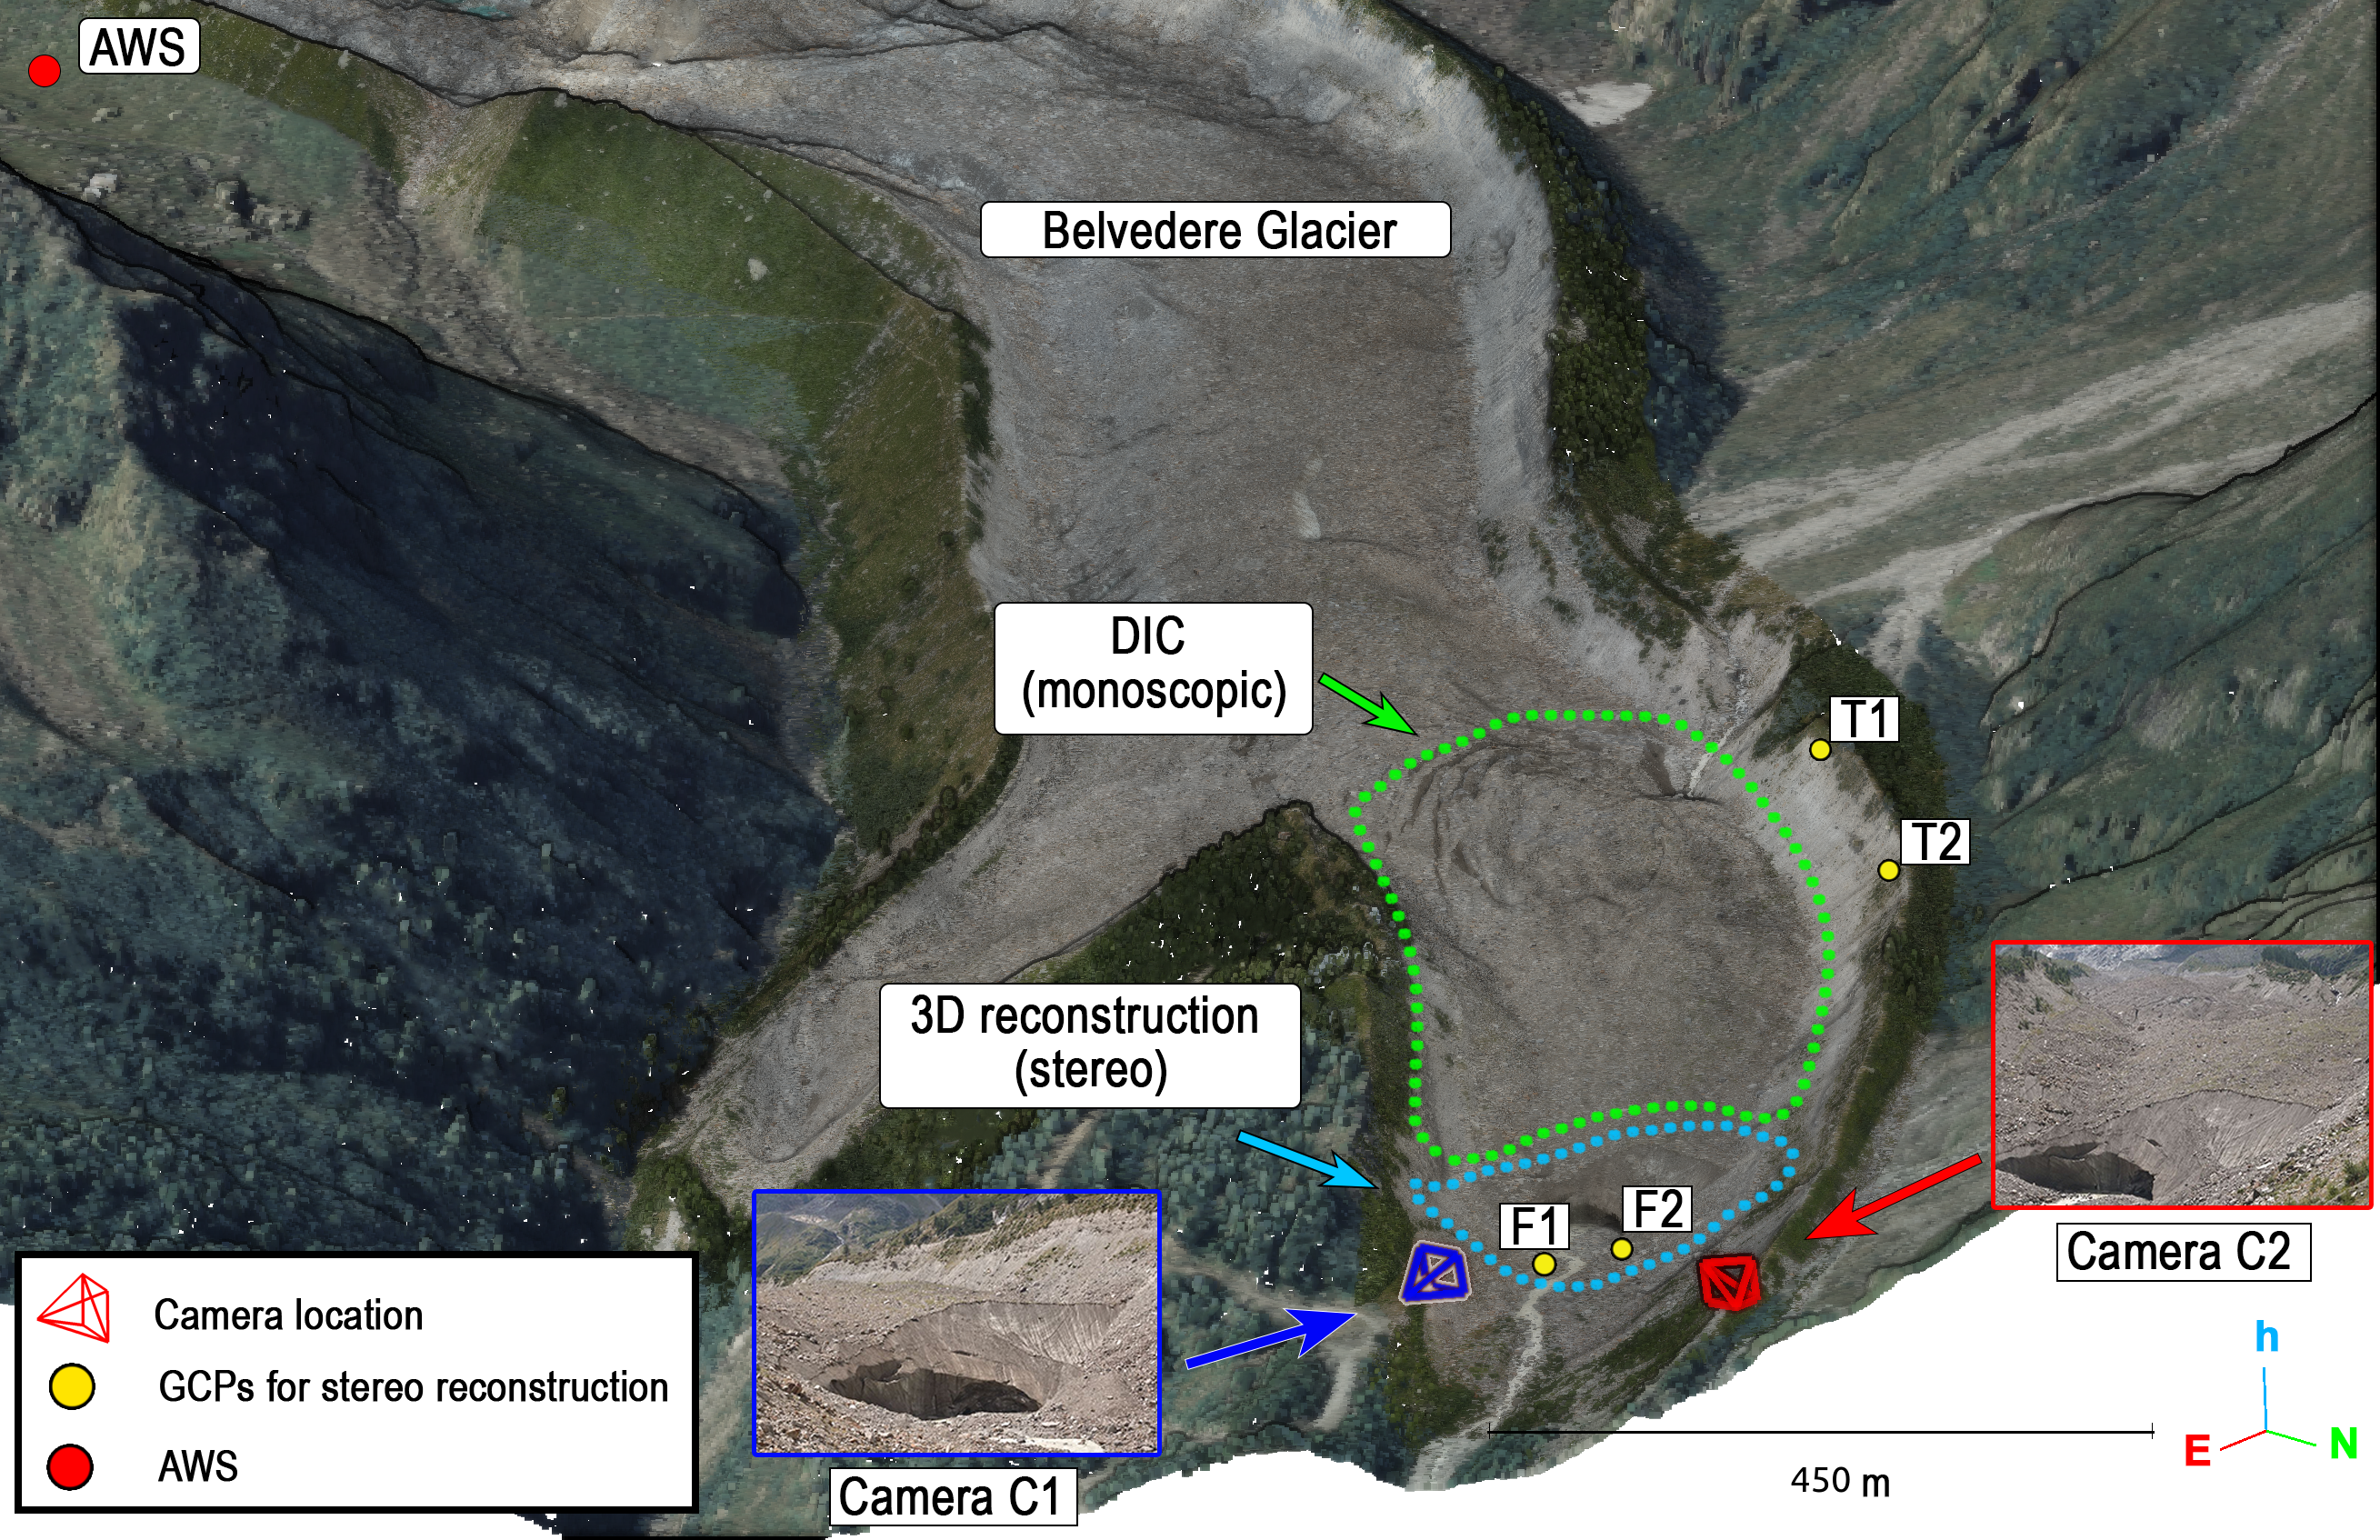
\includegraphics[width=0.67\textwidth]{2_area_of_sudy.png}
  }
  \caption{(a) Map of the Belvedere Glacier, with marked the location of the two cameras C1 and C2, the Automatic Weather Station (AWS) and the Zamboni Zappa Hut;
  (b) The area of study: the stereoscopic reconstruction is focused on the terminal ice cliff (dashed light blue line), while the monoscopic DIC processing from camera C2 image sequence is focused on the upper area of the north lobe (dashed green line).}
  \label{fig:4:studyarea}
\end{figure}

\section{The low-cost stereoscopic system}\label{sec:4:system}

% From last paper
The low-cost stereoscopic system consists of two autonomous and independent monitoring
units. Each unit is includes an off-the-shelf DSLR camera (Canon Eos 1200D), an Arduino
microcontroller for camera triggering, and a Raspberry Pi
Zero with a SIM card for sending images to a remote server via a GSM
network \citep{ioli2023_replicable}.
The instruments are housed in waterproof cases and mounted on tripods anchored to stable
rocks along the glacier moraines.
Power is supplied by a solar panel combined with a sealed lead-acid battery.
The total cost of each unit was less than \texteuro2000, including
camera and lens \citep{ioli2023_replicable}.
The low-cost camera system is described in detail in \citet{ioli2023_replicable}.

The two monitoring stations, labelled as C1 and C2, were installed in summer 2021 on
either side of the north tongue of Belvedere Glacier (\figref{fig:4:studyarea}).
The harsh glacier environment with steep and unstable moraines, often subject to rockfall
due to glacier retreat, constrained the camera installation location at
\SI{\sim230}{\meter} (camera C1) and \SI{\sim350}{\meter} (camera C2) from the terminal
ice cliff, with a strongly convergent pose.
Different lenses were used for the two cameras to achieve the same image scale in
correspondence of the glacier tongue: C1 was equipped with a 24 mm lens, while a 35 mm
lens was used for C2.

\begin{table}
  \centering
  \caption{Summary of the characteristics of the two cameras.
    Fields marked with $^*$ are computed considering the distance between each camera and
    the ice cliff.}
  \label{tab:4:cameras}
  \begin{tabular}{c c c}
    {}              & C1                               & C2 \\
    \hline\noalign{\smallskip}
    Camera          & Canon Eos 1200D
                    & Canon Eos 1200D                       \\
    Sensor          & APS-C
                    & APS-C                                 \\
    Pixel size      & \SI{3.7}{\micro\meter}
                    & \SI{3.7}{\micro\meter}                \\
    Image           & \qtyproduct{6000x4000}{\pixel}
                    & \qtyproduct{6000x4000}{\pixel}        \\
    Lens            & Canon EF 24mm f/2.8 IS USM
                    & Canon EF 35mm f/2 IS USM              \\
    Distance$^*$    & \SI{230}{\meter}
                    & \SI{350}{\meter}                      \\
    Average GSD$^*$ & \SI{3.5}{\centi\meter\per\pixel}
                    & \SI{3.5}{\centi\meter\per\pixel}      \\
    \noalign{\smallskip}\hline
  \end{tabular}
\end{table}

The baseline between the two cameras of \SI{\sim 261}{\meter} ensured a good
viewing geometry because of the large parallax between corresponding points.
However, the baseline comparable to the camera-object distance (base-height ratio close
to \(1\), \tabref{tab:4:cameras}) led to complex affinity-like distortions and occlusions
between corresponding areas in the two images~\citep{Yao_2021}.
Additionally, C1 was positioned at a lower viewpoint compared to C2, due to
site geometry constraints.
Therefore, camera C1 provides a limited view that primarily encompasses the frontal ice
cliff, but does not capture the glacier surface, which is only visible from camera C2.

The stereoscopic system was operating from August 2021 up to December 2022, when it was
temporarily unmounted for ordinary maintenance, and finally mounted again in June 2023.
During the operational period, the system was programmed to acquire two images per day,
but only one image per day was used for the multitemporal processing.
Only daily images taken during the snow-free period between 01/05/2022 and
13/11/2022 were considered.
In this period, the glacier is experiencing the most significant changes, flow velocity
and ablation rates. On the other hand, during winter and spring seasons, the glacier was
covered by snow, making it difficult to extract relevant information from optical images
for tasks such as 3D reconstruction and surface velocity estimation.

% From paper antalya
The low-cost stereoscopic system for continuous monitoring is composed of two independent
units, each housing an off-the-shelves DSLR camera.
Each unit consists in an autonomous monitoring station that provides power supply,
internet connectivity, timing and scheduling of image acquisition, and protection from
the harsh environment.
The station was designed and built adapting to the alpine environment an existing
open-source model developed by Greig Sheridan and published on
GitHub\footnote{\label{foot:greig}Greig Sheridan' Intervalometerator repository:
  \url{https://github.com/greiginsydney/Intervalometerator}}.
A key aspect of the project was to ensure easy assembly and realization of the system to
guarantee future replication or improvement by non-experts.
In the following, we describe in detail the services and the
nominal performances provided by our system that make it worth consideration for
applications in different monitoring contexts. Refer to \figref{fig:4:scheme_foto} for
a descriptive schematic of the whole system showing the components selected for the
Belvedere Glacier case study. The choice of the camera and optics is discussed in Section
XX, as these components are dependent on the domain of use of the
stereoscopic system.

\begin{figure}[h!]
  \centering
  \includegraphics[width=0.6\textwidth]{schema.pdf}
  \caption{Scheme of the proposed acquisition system configuration for a single
    monitoring station. Arrows indicate the direction of signal initiation. Image adapted
    from Greig Sheridan's repository.}
  \label{fig:4:scheme_foto}
\end{figure}

\subsection{Power supply}\label{Power_supply}
Each monitoring unit has its autonomous power supply line (yellow arrows in Figure
\ref{fig:4:scheme_foto}) provided by a solar panel combined with a sealed lead-acid
battery. An MPPT (Maximum Power Point Tracker) charge regulator directly connects with
the unit's internal circuit, providing a regular current supply to the battery
and the load and exploiting all the power generated by the panel. This regulator prevents
any excess current that may damage the connected device, thus increasing the reliability
of the system. Its battery life-saving algorithm modulates the load disconnection level
so that a nearly 100\% recharge is achieved about once every week and, in case of battery
discharging, the whole system is switched off until 100\% recharge of the battery is
achieved.
The whole monitoring system is designed to minimise power consumption, e.g., by powering
off devices responsible for the highest power consumption when not needed.
An estimation of the system's energy consumption guided the choice of the components of
the power supply line. Specifically, the battery and the associated panel must be
accurately dimensioned for the system's purpose. To this end, the Photovoltaic
Geographical Information System (PVGIS) \citep{pvgis}, a tool provided by the European
Commission, was used. PVGIS can estimate the performance of off-grid photovoltaic systems
according to the installation site and it is supported by a database and algorithms for
calculating solar radiation. Tuning the parameters for the Belvedere Glacier location and
the system consumption, we ended up with the specifications of solar panel power of 30 W
and battery voltage of 12 V and capacity of 10 Ah. Some compromises were made, accepting
that the system would not be sufficiently powered in the months with lowest solar
radiation (November, December, January, and February). {\color{red} further details on
    PVGIS simulations for the Belvedere Glacier case study re given.}

\subsection{System control and scheduling}\label{Control}

\begin{figure}[ht!]
  \centering
  \includegraphics[width=0.6\textwidth]{board.jpg}
  \caption{Stripboard on which are soldered the main components of the internal
    circuit: capacitors (1), voltage regulators (2), real-time clock with coin-cell
    battery (3), Arduino Pro Mini (4), optoisolators (5), and Raspberry Pi Zero W (6).
      {\color{red} Add pic of new board}}
  \label{fig:4:circuit}
\end{figure}

The internal electronic circuit (red box in \figref{fig:4:scheme_foto}) of the
monitoring unit is the only load connected to the power supply and is responsible for all
the system's control and scheduling functionalities.
Its components are a real-time clock (number 3 in \figref{fig:4:circuit}) with a 12
mm
coin-cell backup battery, an Arduino microcontroller (Pro  Mini 328 3.3V 8MHz, number 4
in \figref{fig:4:circuit}), a Raspberry Pi Zero W with 128 GB SD memory card (number
6 in \figref{fig:4:circuit}), and minor elements for connections, isolation (capacitors and optoisolators numbers 1 and 5 in \figref{fig:4:circuit}), and voltage regulations (numbers 2 in \figref{fig:4:circuit}).
The circuit was realized manually by soldering wires and components on a stripboard (see \figref{fig:4:circuit}).

The Arduino communicates through an SPI (Serial Peripheral Interface) bus with an
accurate real-time clock to schedule its actions: waking the camera, firing the shutter to take a photo, and turning on/off the Raspberry. 
The Raspberry is able to access the camera images and transfer them to a remote server via internet connectivity. 
A large storage memory is added to the unit to save photos before remote transferring. 
The Raspberry also provides a web-based, user-friendly interface
(\figref{fig:4:web-interface}) to configure and monitor the system remotely
\citep{greig}.
An I2C (Inter Integrated Circuit) bus and digital pin connections enable higher-level
communication between these two boards. Among the minor components, we mention the role
of the three voltage regulators. They allow each unit to be powered at the appropriate
voltage and current: starting from the 12 V in input, one delivers 3.3 V and 500 mA to
the Arduino, one 5 V and 2.5 A to the Raspberry and its hat, and the other 7.5 V and 2.4
A to the camera. The Arduino controls the 5V regulator of the Raspberry to reduce
quiescent power consumption when the Raspberry board is off.

Acquisition of a defined number of images, camera triggering and timing, and sending of
images to a remote server can be scheduled thanks to adequate programming of a cyclic
executive program in C++ for Arduino and  of services executing automatically Python
scripts for the Raspberry.
All the monitoring station activities can be remotely scheduled from the terminal or a
user-friendly web interface \citep{greig}. This useful feature allows one to change the
settings and check the behaviour of the system, avoiding the need for manual
intervention. The Raspberry uses the gPhoto2, a Python-based protocol developed to
specifically interact with popular cameras’ firmware, to communicate with the camera and
access the new photos. The  web-based interface service is based on NGINX and Gunicorn,
open-source software for web servers. The interface (\figref{fig:4:web-interface})
consists of a web page accessible with credentials and provides a summary of the system
state and the exact time of the last operations (time of the last shot and the last
upload of images), temperatures of the components, previews of the last images, buttons
to wake up the camera, take a preview photo and schedule the system routine (time and
number of photo acquisition, wake-up time of the Raspberry) and some camera settings.

\begin{figure}[h!]
  \centering
  \includegraphics[width=0.8\textwidth]{web_interface.png}
  \caption{Example of some of the pages of the web-based interface to remotely control
    the monitoring units.}
  \label{fig:4:web-interface}
\end{figure}

All the components were chosen because of their low power consumption and their
inter-compatibility. The circuit is robust against power losses due to battery
discharging and is able to auto-recover when power is regained. A low energy consumption
policy is also followed in selecting the scheduling. The camera is switched on only
during the data capture activity. The Raspberry is switched on only once per day when the
connection with the remote server and image transfer is scheduled.

\subsection{Connectivity}\label{Connectivity}
Internet connectivity is crucial to transfer images and to control the units remotely. To
this end, the Raspberry is equipped with the SIM7600E-H 4G hat by Waveshare. The module
supports 4G/3G/2G communication via a SIM card. Raspberry and hat operations are the most
expensive in terms of power consumption. For this reason, the board is switched on only
once a day for a limited period of time, which is kept adequately low to be sustainable
for the system power supply but still sufficient for transferring new images to the
server. We adopted IoT (Internet of Things) SIM cards provided by the multi-operator
service Emnify \citep{emnify}, as it offers the ability to connect to the best-quality
cellular network available and includes flexible and customizable data plans.
Remote access to the devices is allowed by a VPN (Virtual Private Network).
The service costs \texteuro33 per month for a data plan with 6 GB.

\subsection{Case and protection}\label{Case and protection}
The majority of the components need to be protected. Therefore, a solid and compact case
that allows keeping all the parts (with the exception of the solar panel) in the same
location is desirable for the functioning of the system and for convenient
transportation, installation and maintenance. The case should also satisfy the thermal
insulation requirements according to each component's working temperature range. The case
should also be waterproof and robust against different and harsh weather conditions but,
at the same time, provide access for connecting the solar panel and taking pictures. Our
choice was an HPRC 2250 lightweight, waterproof resin case with internal insulating foam.
The foam was found to be useful in enhancing the temperature seal and stabilising the
location of some components, preventing unwanted movements. Holes were drilled in the
case: one sealed with a UV filter of 82 mm to allow the camera to take shots, two others
to give access to the solar panel wires, and others to fix the system to a tripod. The
internal case dimensions (236x182x155 mm) posed a significant challenge in accommodating
all the components inside. In particular, the camera lens dimensions were constrained by
space availability.

\subsection{General performances}\label{General_performances}
The system was subject to several tests before being used in its final application at the
Belvedere glacier site. During these tests, the system proved to be autonomous, robust to
sudden shutdowns, cold-resistant, water-resistant and self-sufficient for a prolonged
period of time with no direct sunlight on the solar panels. Specifically, in the absence
of sunlight, the battery is able to power the system for about nine days before it is
completely discharged. Battery voltage and temperatures of components were monitored,
simulating the absence of solar radiation and low environmental temperatures. See Figure
\ref{fig:4:nominal_performance} for the performances of the system during these tests.
\begin{figure}[h!]
  \centering
  \includegraphics[width=.5\textwidth]{nominal.png}
  \caption{Battery voltage and temperature of boards with and without the solar panel
    during a period of tests. Starting from a fully charged condition, the system was
    kept without solar panel at around 2 °C for the first six days. After nine days, the
    battery was fully discharged and the system was reconnected to the panel and exposed
    to solar radiation.}
  \label{fig:4:nominal_performance}
\end{figure}

\subsection{Camera and lenses}\label{camera_lenses}
The choice of the DSLR camera and of the optics can be considered application-dependent.
Therefore specifications regarding these components are reported in reference to the
Belvedere glacier case study. Each monitoring station was equipped with a DSLR camera
Canon EOS 2000D, with 24.1 MP CMOS \mbox{APS-C} sensor. This model was chosen because of
the limited costs, the high image resolution and its compactness, as it must fit inside
the case. Additionally, another fundamental requirement was camera compatibility with the
gPhoto2 software. In the installation inside the system case, the traditional
rechargeable battery was replaced by a special battery (”fake battery”) equipped with a
power supply cable, which provides a voltage of 7.5 V from the circuit. The camera is
attached to a sliding plate able to vary, with a limited range, and then fix the position
of the camera on the longitudinal axis. Screws fix the camera to the plate and the plate
to the case.

The two stations were installed respectively at \SI{\sim 180}{\meter} and \SI{\sim 340}{\meter} m distance to
the glacier terminus (see \figref{fig:4:studyarea}), avoiding the steep moraines
of the glacier, often prone to collapses and landslides. Therefore, a wide baseline of
\SI{\sim 260}{\meter} occurs between the two sensors.
The final positioning of the two cameras was decisive in the choice of optics.
In fact, to ensure comparable Ground Sample Distance (GSD) of the images (\SI{\sim 3}{\centi\meter\per\pixel}), lenses with different focal lengths were employed.
In particular, a Canon EF 24 mm f/2.8 IS USM and a Canon EF 35 mm f/2 IS USM were used
respectively for Camera 1 (stream-wise right) and Camera 2 (stream-wise left).

\subsection{Camera installation}\label{Monumentation}

Monumentation of the two cameras at the Belvedere Glacier site was achieved by choosing
two large stable rocks along the moraines.
Each camera is supported by an aluminium topographic tripod system anchored with steel
dowels and cables to the rocks (\figref{fig:4:final_installation}b).
A central steel tie rod keeps the system in a fixed position.
The choice of an agile monumentation was aimed at having a system that can be rather
easily assembled on site (and also disassembled, if needed), also in a harsh environment,
with limited costs and time.
To install the cameras, in fact, all the equipment was carried in backpacks along the
moraines, sometimes without a marked walking path (e.g., in the case of the stream-wise
left camera).
As a drawback, the analysis of the acquired photos revealed a non-optimal stabilization
of the two cameras.
In fact, small rotations, especially around the vertical axis, and vibrations, mostly
induced by the wind, were experienced.
Though, a perfectly stable monumentation in a mountain environment is hardly achievable.
Therefore, it is not possible to assume the camera orientation as stable a priori, but
camera orientation must be estimated based on some Ground Control Points (GCPs) located
on the ground in stable areas.

It is worth mentioning the performances of the system in terms of costs: our  monitoring
system can be fully reproduced with an average cost of \texteuro2000 per station
(November 2023), including camera (\texteuro400), lens (\texteuro500) and material for
the on-site installation (\texteuro150).
In comparison, commercial time-lapse cameras are expensive
(e.g., PhotoSentinel\footnote{PhotoSentinel: \url{https://photosentinel.com/} (accessed
  on 15/11/23)} cameras cost more than \$ 5,000.00) and hardly customizable.
The final prototype of the monitoring station is shown in Figure
\ref{fig:4:final_installation}.

\begin{figure}[h!]
  \centering
  \includegraphics[width=.2\columnwidth]{finale1.pdf}
  \includegraphics[width=0.3\columnwidth]{centralina.jpg} \\
  \centering{(a)\hspace{30mm}(b)}\\ \vspace{1mm}
  \caption{(a) Picture of the monitoring unit prototype installed for tests at the
    Belvedere Glacier site. (b) Picture of the final monumentation of the camera
    installed on
    the stream-wise right moraine. {\color{red} TODO: change picture with the final
        installation}}
  \label{fig:4:final_installation}
\end{figure}

\section{Datasets}\label{sec:4:datasets}

\subsection{stereoscopic image sequences}\label{sec:4:stereo}

During the snow-free study period (from 1/05/2022 to 13/11/2022), both camera C1 and
camera C2 were able to acquire images every day, for a total of 197 images. However, 39
images were discarded due to bad weather conditions, such as rain, low clouds, or fog,
resulting in 158 days with valid data for stereo and monoscopic processing

  {\color{red} TODO: write about the images sequence 2022 and 2023}

\subsection{UAV surveys}\label{sec:4:uavsurveys}

Two UAV flights, spaced by a 10-days interval, were conducted in summer 2022 to acquire
ground truth data for assessing the proposed methodology.
The first UAV flight, labelled as UAV-A, was carried out on 28/07/2022 with a DJI
Matrice 300 RTK quadcopter and a DJI Zenmuse P1 camera with a 35 mm lens.
During the survey, 436 images were captured, encompassing both nadiral and oblique
perspectives.
Additionally, 19 Ground Control Points (GCPs) were measured using a combination of a
total station and Differential GPS (DGPS), employing a topographic-grade
GNSS receiver.
The GCPs included both artificial targets and natural features.
During the flight, the UAV was equipped with an on-board RTK GNSS receiver, enabling the
acquisition of camera projection centers with decimetric accuracy.
The photogrammetric block (\figref{fig:4:uavblocks}a) was processed with the commercial
software package Agisoft Metashape \citep{agisoft} by using 14 GCPs and 5 Check Points
(CPs) to evaluate the block accuracy.
The global RMSE evaluated on the CPs was equal to 4.0 cm.

The secondo UAV flight, UAV-B, was carried out on 05/08/2022 with a DJI Phantom
4 RTK, focusing on a smaller portion of the northern lobe of the Belvedere Glacier.
However, due to technical constraints, \textit{moving} GCPs located inside the
glacier body were not measured again.
Therefore, only the fixed targets located outside the glacier were employed.
Among these, 8 targets were designated as GCPs, while the remaining 4 were used as CPs.
The photogrammetric block encompassed 428 nadiral and oblique images, which
were processed using Agisoft Metashape (\figref{fig:4:uavblocks}b).
A global RMSE of 7.5 cm was obtained on the 4 CPs.

\begin{figure}
  \centering
  \subcaptionbox{\label{fig:4:uavblocks:A}}{
    \includegraphics[width=.45\textwidth]{2_UAV-A_280722.png}
  }
  \subcaptionbox{\label{fig:4:uavblocks:B}}{
    \includegraphics[width=.45\textwidth]{2_UAV-B_050822.png}
  }
  \caption{(a) UAV-A block and (b) UAV-B block processed with Agisoft Metashape. The
    flags represent the targets used either as GCPs in the BA or as CPs to evaluate the
    quality of the photogrammetric block.}
  \label{fig:4:uavblocks}
\end{figure}

\subsection{Meteorological monitoring station}\label{sec:4:meteostation}

To analyze the correlation between the Belvedere Glacier dynamics and
external environmental variables, data measured from an Automatic Weather Station (AWS)
located close to the Zamboni Zappa Hut were used.
The AWS is located at an altitude of \SI{2075}{\masl} and at a distance of
2 km from the area of study.
In our study, we analyzed mean daily values of air temperature, precipitation and
incoming solar radiation from 01/05/22 to 15/11/22.

\section{Methodology}\label{sec:4:methodology}
This chapter outlines the methodology developed to monitor the evolution of the Belvedere
Glacier northern lobe.
The daily images were processed using a framework consisting of two parallel processing
chains (\figref{fig:4:workflow}):
(i) a photogrammetric-based stereoscopic approach;
(ii) a DIC-based monoscopic approach.
The daily stereo pairs were used to generate 3D models of the glacier terminus,
enabling the estimation of ice volume loss on a daily basis by computing point cloud
differences along the main flow direction.
However, due to limited overlapping views of the two cameras, the stereoscopic approach
primarily provides a 3D reconstruction of the terminal ice cliff (dashed-blue area in
\figref{fig:4:studyarea}b).
Consequently, deriving the 3D surface velocity field of the glacier solely from
photogrammetry was not feasible.
The image sequence captured by camera C2, offering a higher viewpoint and broader
coverage of the glacier surface, was employed to determine the glacier's surface velocity
over a larger area of the north lobe of the Belvedere Glacier (dashed-green area in
\figref{fig:4:studyarea}b).

\begin{figure*}[ht]
  \centering
  \includegraphics[width=154mm]{3_general_workflow.png}
  \caption{General workflow with two parallel processing chains involving stereoscopic
    reconstruction of terminal ice cliff from stereo-pairs of images to derive ice volume
    losses at the glacier terminus and glacier retreat and monoscopic digital-image
    correlation to derive surface velocities.}
  \label{fig:4:workflow}
\end{figure*}

\subsection{Image selection}\label{sec:4:imageselection}

Once the acquired images have been received from the monitoring system, an
automatic selection of the images was performed to exclude the ones acquired in rainy,
foggy, or poor lighting conditions.
This selection was based on the analysis of images median
entropy~\citep{tsai2008entropy}:
the images with a low value over the entire image were rejected.
Additionally, a visual inspection was performed on the entire image dataset.
The inspection had the following objectives:
(i) selecting only one image per day;
(ii) rejecting poor quality images that were not automatically rejected,
and images in which the fixed targets placed along the moraines were not visible;
(iii) detecting of sudden changes in the morphology of the glacier
terminus (e.g., icefall).

\subsection{Camera calibration}\label{sec:4:cameracalibration}

Each camera was mounted with all its electronics inside a waterproof case and protected
by a neutral filter that was glued to the case and fixed in front of the cameras.
Since the filter introduced additional distortion, the cameras need to be calibrated
inside the boxes to reproduce the final setup.
Therefore, a two-step approach was taken: first, a 120 cm x 70 cm calibration board with
a checkerboard printed on it was used to estimate an initial set of parameters for the
interior orientation \citep{zhang_flexible_2000}.
To this end, the cameras were mounted on tripods inside their cases while the calibration
board was moved and rotated in front of the camera to simulate a convergent hemispheric
acquisition.
For each camera, about 30 images were collected and processed in Agisoft Metashape to
obtain a first estimate of the interior orientation.
However, the average camera-to-panel distance was much smaller than the actual
camera-to-glacier distance.
Therefore, a refinement of the calibration was performed in-situ by incorporating the
stereo pair acquired by the cameras on 28/07/22, within the UAV-A block, carried out on
the same day.
This block was processed with Agisoft Metashape to refine the interior camera
orientation of the stereo cameras, aided by the increased robustness of the block given
by the additional matches between the two images taken by camera C1 and C2 and the UAV.

An additional challenge was represented by camera interior orientation stability over
time.
From experimental evidence, the interior orientation parameter that suffered the most
because of temperature variations that occurred in mountain environment
was the camera principal distance \citep{Elias2020}, while the other parameters
remained more stable during time.
To mitigate the impact of temperature-induced variations, it was crucial to incorporate
camera self-calibration during the stereoscopic processing at each epoch to refine the
pre-calibrated principal distance.

\subsection{Camera stability and GCPs}\label{sec:4:stability}

Since the two cameras were mounted on topographic tripods, the stability of the cameras
was not perfectly guaranteed. In particular, the two cameras experienced small vibrations
around their pivots due to wind gusts.
On the other hand, the position of the cameras was constrained by topographic heads that
kept the position of the camera center constant to the centimeter level.
Therefore, the baseline of the cameras can be reasonably considered as constant, with a
value of \SI{261.55}{\meter}.
On the other hand, camera angular vibrations implied that the relative orientation of the
cameras must be estimated at each epoch.
Moreover, to fix the world reference system over time, absolute orientation of the
stereo model was required.
To this end, the position of the cameras was measured in-situ using a topography-grade
GNSS receiver in RTK.
In addition, four GCPs were materialized with plastic targets, anchored to stable rocks
in front of the terminal ice cliff and along the streamwise left
moraine (\figref{fig:4:studyarea}a).
While the minimum requirement to estimate a Helmert transformation would have been just
the two cameras' location and one one GCP, having a redundant number of GCPs overcomes
the possibility that on some days not all GCPs were clearly visible in the images due 
to low clouds or fog.
Additionally, GCPs can be included into the BA to refine the cameras' interior
orientation, and in particular the camera's focal length.

As the cameras are subjected to slight rotations, the image coordinates of the GCPs'
projections must be detected at each epoch.
To this end, a feature tracking routine was developed based on the ImGRAFT TemplateMatch
method~\citep{Messerli2015} to track a GCP on all images in the time-series by DIC. 
This involves defining a template on a reference image and search 
orientation correlation algorithm~\citep{fitch2002_OC}, which is more robust against illumination changes compared to normalized cross-correlation and achieves sub-pixel accuracy~\citep{Dematteis2021,Heid2012_evaluation_xcorr}.

\begin{figure}
    \centering
    \includegraphics[width=1\textwidth]{tracking_gcp.png}
    \caption{Example of template matching used to track GCPs on a
        monocular image sequence. The green square represents the
        template on the reference image that is searched in all the other
        images of the sequence.
        The red cross marks the estimated position of the center of the
        template in a new
        image.}
    \label{fig:4:templatematch}
\end{figure}

\subsection{Stereoscopic image processing workflow}\label{sec:4:stereoworkflow}

\begin{figure}
  \centering
  \includegraphics[width=.6\textwidth]{3_stereo-workflow.png}
  \caption{Scheme of the stereoscopic workflow performed with ICEpy4D. At a generic epoch
    \(i\), new features are extracted and matched.
    At the same time, features from the previous epoch \(i-1\) are tracked on the current
    epoch images. After geometric verification, features successfully
    matched are used for 3D scene reconstruction. Point clouds obtained on
    different days are used to compute ice volume differences and glacier
    retreat.}
  \label{fig:4:stereo-workflow}
\end{figure}

For the daily stereoscopic reconstruction of the glacier snout, a Python-based toolkit
ICEpy4D was developed (ICEpy4D code is available in the repository
\url{https://github.com/franioli/icepy4d}).
ICEpy4D allows for solving different steps of scene reconstruction
(\figref{fig:4:stereo-workflow}). In particular, the main steps consist of:
(i) finding corresponding points by deep-learning feature matching;
(ii) tracking features on sequence of images acquired from the same camera;
(iii) performing 3D scene reconstruction and point cloud post-processing.
All the processing was carried out with a mid-class workstation equipped with a 20-cores
i7-12700 CPU, 32~Gb of DDR5 RAM and a GPU NVIDIA RTX A2000 12~GB.

\subsubsection{Wide-baseline image matching}\label{sec:4:matching}

To find corresponding points, the combination of DL feature-matching algorithms
SuperPoint \citep{DeTone_2018} and SuperGlue \citep{sarlin2020superglue} was used and
fully integrated into ICEpy4D package.
SuperPoint is a Convolutional Neural Network (CNN) with an encoder-decoder
structure, which detects interesting points and computes 256-value descriptors in a
single forward pass.
\citet{DeTone_2018} trained SuperPoint to detect corner-like features first using corners
of synthetic shape datasets as ground truth.
They employed a self-supervised approach by applying random homographies to warped
copies of the input training images and combining the results \citep{DeTone_2018}.
SuperGlue is an attention-based graph CNN used for local feature matching.
It was specifically designed to match SuperPoint features based on their descriptors.
\citet{sarlin2020superglue} trained SuperGlue in a supervised manner and published two
different sets of weights: one for indoor environments and another for outdoor
environments.
The outdoor environment model was trained on the Megadepth dataset
\citep{Li_Snavely_2018_MegaDepth}.

The SuperPoint and SuperGlue models were not fine-tuned to ensure the replicability of
the proposed pipeline in different scenarios, without the need for a
dedicated ground truth dataset.
Acquiring a ground truth dataset may be can be challenging, especially for natural
scenarios and mountain environments.
Typically, generating datasets for training wide baseline matching requires collecting a
substantial number of image sequences with a normal baseline and artificially creating a
wide baseline by skipping intermediate images.
However, this approach would demand numerous field campaigns to capture series of UAV
images under different environmental conditions and throughout various seasons, making it
generally unfeasible.
Moreover, the matching results obtained with the Belvedere stereo pairs were already
satisfactory using pre-trained weights for outdoor environments without any fine-tuning
(see results in \secref{sec:4:res_matching}).

Since feature matching was performed on a GPU, which has limited memory, it was necessary
to decompose the full-resolution images into smaller tiles and match pairs of tiles one
after the other.
Therefore, a two-steps approach was implemented: first, a matching is performed with
SuperPoint and SuperGlue on downsampled images. Subsequently, the
full-resolution images were subdivided into regular tiles, and only the tiles that had
corresponding features in the low-resolution images were selected as candidates for a
second matching step.
In the second step, the selected tiles were matched using the same procedure as before.
The features matched in each tile were then reassembled to recover their image
coordinates on the original image for geometric verification.
Incorrectly matched keypoints, which did not satisfy the epipolar constraint, were
rejected using Pydegensac~\citep{Mishkin2015_pydegensac}, by imposing a maximum
re-projection error of 1.5 px.

\subsubsection{Tracking points over epochs}\label{sec:4:tracking}

\begin{figure}
  \centering
  \includegraphics[width=0.8\textwidth]{3_tracking.png}
  \caption{Scheme of feature tracking in stereo-cameras sequence. At each epoch, new
    features are matched on the stereo pair (horizontal lines), but also tracked from
    previous epochs (oblique lines).
    At epoch 0, the matches are only the corresponding features matched
    between	current the stereo pair (red triangles).
    At epoch 1, the valid matches are the new corresponding features matched (green
    triangles) plus the successfully tracked features from epoch 0 (red triangles).
    The same holds for epoch 2, where the matches are the new
    corresponding features (yellow pentagons), plus the features tracked from both epoch
    0 and 1.}
  \label{fig:4:tracking}
\end{figure}

Matched points are tracked over time on single camera image time series
(\figref{fig:4:tracking}).
This procedure led to two main advantages: (i) increasing the number of matches
at every epoch; (ii) obtaining a time-series of corresponding points that can be
triangulated to derive their 3D coordinates over time.
For brevity, images are labeled with the camera labels \(C1\) and \(C2\), while a
superscript indicates the acquisition epoch.
At a generic epoch \(i\), keypoints were detected and
matched between images \(C1^i\) and \(C2^i\) with the procedure described
in \secref{sec:4:matching}.
SuperPoint features were then extracted on \(C1^{(i+1)}\) and \(C2^{(i+1)}\).
Valid matched features from \(C1^i\) were tracked to \(C1^{(i+1)}\), by matching their
descriptors with the SuperGlue algorithm.
The same holds for camera \(C2\).
If a matched feature at epoch \(i\) was tracked successfully both from images
\(C1^i\) to \(C1^{(i+1)}\) and from images \(C2^i\) to \(C2^{(i+1)}\), then this feature
was considered a valid match also for epoch \(i+1\) and merged to the new corresponding
features detected at epoch \(i+1\).
Duplicate features (e.g., a feature that was successfully tracked from epoch \(i\) to
epoch \(i+1\) but also matched again at epoch \(i+1\)) were removed and a new geometric
verification was carried out to reject outliers.

\subsubsection{3D scene reconstruction}\label{sec:4:3dreconstruction}

At each epoch, the reconstruction of the terminal ice cliff was carried out using ICEpy4D
in two main steps: (i) relative-absolute orientation, and (ii) bundle adjustment.
In the first step, matches between each stereo-pair were utilized to estimate the
relative pose of the two cameras, based on the camera's pre-calibrated intrinsic matrix.
Subsequently, the absolute orientation was determined by calculating a Helmert
transformation, considering the cameras' locations and the available GCPs.
In the second step, a full BA was performed to refine the relative-absolute solution. For
this purpose, the Agisoft Metashape software package was employed via its Python API.
The choice of Agisoft Metashape was driven by its support for GCPs, the possibility to
assign different a-priori weights to observations, and the availability of a Python API,
enabling the software to be run from a Python routine in headless mode.
The Metashape BA was seamlessly integrated into ICEpy4D, enabling the entire workflow
chain to run automatically without any interaction with the GUI.

During the BA, the cameras' locations and the available GCPs were used as observations.
A centimetric a-priori accuracy was assigned to the world coordinates of the GCPs.
A centimetric accuracy was also given to the camera locations to constrain their
positions, while still allowing for an estimation of the cameras' rotations.
Additionally, during the BA process, the principal distance of the
two cameras was refined by self-calibration based on the available GCPs, while the
remaining interior orientation parameters were kept fixed at their pre-calibrated values.

The dense reconstruction of the ice cliff terminus was again carried out using the
Agisoft Metashape API.
In fact, although Agisoft Metashape couldn't perform feature matching with wide baselines
due to its reliance on hand-crafted features, it was effective in performing dense
matching through semi-global matching
algorithms~\citep{Hirschmuller2012}, when accurate camera poses were available for image
rectification.
Depth maps were generated from full-resolution images (i.e., the highest
quality parameter in Agisoft Metashape) with mild filtering.
The estimated depth maps were then used to reconstruct a dense point cloud and a
triangulated mesh.


\subsection{Volume variation estimation}\label{sec:4:volumevariation}

\begin{figure}
\centering
  \includegraphics[width=1.0\linewidth]{3_dod_scheme.png}
  \caption{Scheme of Dem of Difference (DOD) approach used to compute volume variations
    at the glacier terminal ice cliff.
    Two point clouds built at epoch i and i+dt (we used dt=5 days to increase the
    signal-to-noise ratio), were rasterized to a vertical Y-Z planes, with normals
    parallel to the glacier flow direction (X direction).
    Before rasterization, the point clouds are clipped with the same convex polygon in
    the Y-Z plane (red line).
    The colors of the grids represent the depth of each cell of the two rasters along the
    X direction (i.e., the distance along X from a reference plane).
    Volume variation was computed by DOD of the two rasters along X.}
  \label{fig:4:dod_scheme}
\end{figure}

The daily variation of ice volume was determined by calculating the DEM of Differences
(DOD) along the streamwise direction. A local reference system was established by
defining the X-direction as the streamwise direction, the Z-direction as the geodetic
height, and the Y-direction to complete the right-hand reference system.
The point clouds of two different epoches were rasterized to a reference YZ plane,
corresponding to the frontal view of the terminal ice cliff, using a grid step of 0.3
meters, while maintaining the same raster origin and extent (i.e., the two point clouds
were first clipped with the same convex polygon).
The volume change between two epochs was then calculated by differentiating the
two rasters cell-by-cell (\figref{fig:4:dod_scheme}).
To account for possible incomplete coverage and holes in the 3D reconstruction, which may
result in volume underestimating, the computed volume difference was normalized by the
percentage of filled cells (i.e., cells with at least one point in the original point
cloud) in both rasters.
The normalization was computed as in Eq.~\ref{eq:4:volumevariation}:

\begin{equation}
  dV_{\text{norm}} = dV \times
  \frac{n_{\text{filled}}}{n_{\text{total}}}
  \label{eq:4:volumevariation}
\end{equation}

where \( n_{\text{filled}} \) is the number of filled cells in both the rasters and \(
n_{\text{total}} \) is the total number of cells within the clipping polygon.
During the considered study period, the percentage of filled cells in the rasterized
point clouds of the terminal ice cliff ranged from 90\% to
98.8\%, with a mean value of 96.8\%.


\subsubsection{Temporal lag between point clouds for volume and velocity estimation}
\label{sec:4:timelag}

To estimate volume variation and surface velocity, the point clouds were processed using
pairs spaced 5 days apart.
This interval was selected based on the available open-data acquired by Ioli et al. with
historical aerial datasets and in-situ annual photogrammetric UAV surveys on the
Belvedere Glacier between 1977 and 2022~\citep{Ioli2022,ioli_2023_zenodo,Degaetani2021}.
Given a decimetric accuracy of the stereo point clouds (see the results presented
in \secref{sec:4:res_uav_validation}), a 5-day interval was considered appropriate to
achieve a good signal-to-noise ratio.
Therefore, each point cloud acquired on a particular day was compared to that captured
5 days earlier for volume differences computation.
However, in case of adverse weather conditions which hindered stereo reconstruction and
resulted in the unavailability of a point cloud on a certain date, the closest one
acquired within a range 5 to 7-days earlier was chosen as a substitute.
This approach ensured a balance between preserving temporal resolution and minimizing
data gaps caused by unfavorable weather conditions.

To ensure consistency between volume variations and surface velocities, the same pairs of
days utilized for estimating volume differences from point clouds were also employed for
selecting pairs of images to compute surface velocities using DIC on monoscopic image
sequences (see \secref{sec:4:dic}).

\subsection{Automatic extraction of ice cliff top edge}
\label{sec:4:topedge}
To calculate the glacier retreat over time, the top edge of the ice cliff was chosen as a
reference point.
This decision was made because the top edge remained rather stable and experienced
limited changes in morphology compared to the rest of the terminal ice cliff, which is
often affected by deformation and other processes that altered its shape, such as ice
block collapses.

The top edge of the ice cliff was automatically extracted from point clouds, by
exploiting geometric features of each point with respect to its neighborhood
~\citep{Hackel2016}.
To identify elongated features situated at the edges of the ice cliff within the point
cloud, the linearity and normal change rate were computed for each point with respect to
a neighborhood sphere of radius 2 m. By employing empirically determined thresholds
specifically tailored to the study site, these geometric properties facilitated the
identification and extraction of the top edge of the glacier terminus from the point
cloud data.

\subsection{Digital Image Correlation from single cameras}
\label{sec:4:dic}
DIC allows for determining the displacement of an image patch between two images (master
and slave) of the same scene and acquired at different epochs by the same camera. The
displacement \(d\) is obtained as  (Eq.~\ref{eq:4:dic}):

\begin{equation}
  d = \text{argmax}_{(r,q)} S(A(i,j),B(i+r,j+q))
  \label{eq:4:dic}
\end{equation}

where \(S\) is a similarity function, \((i,j)\) are the coordinates of the master patch
\(A\), and \((r,q)\) are the coordinates of a search area around the slave patch \(B\).
In our study, we adopted the open-source Local Adaptive Multiscale image Matching
Algorithm (LAMMA) written in Matlab \citep{Dematteis2022}.
LAMMA adopts a hierarchy structure of patch grids of increasing spatial resolution and
uses locally-adaptive search area sizes, according to the displacements already
obtained in the neighboring region.
LAMMA allows faster computation and reduces the occurrence of outliers compared to
traditional DIC processing \citep{Dematteis2022}. As a correlation function, we used the
cosine similarity applied to orientation images \citep{Dematteis2021}, which is less
sensitive to changes in the shadow pattern and it is known to perform well in glacier
environments \citep{Heid2012_evaluation_xcorr}.

We applied DIC to the undistorted images which were corrected according to the interior
orientation parameters estimated at every epoch within stereo BA.
Moreover, assuming a zero-translation of the camera perspective centers, but only small
rotations (\secref{sec:4:stability}), the transformation between the image plane at an
arbitrary epoch with respect to a reference one (named \textit{master}) is
described by a homography transformation.
As master image, we adopted the image taken on 28/07/2022, which was
coeval with the DSM built from the UAV-A survey.
All the other images acquired were warped to be coregistered to the master image,
by computing a homography transformation \(H\) (Eq.~\ref{eq:4:homography}):

\begin{equation}
  H = KRK^{-1}
  \label{eq:4:homography}
\end{equation}

where \(K\) is the camera intrinsic matrix and \(R\) is the relative
rotation between the image planes \citep{forstner2016}.
The relative rotation \(R\) between the camera pose at a generic epoch and the pose of
the master camera was known from the stereo processing.

The same image pairs used for volume  variation computation, spaced by a time lag of 5
days, were selected for DIC~(\secref{sec:4:timelag}).
The resulting displacement maps on the image plane, in pixel units, were finally
post-processed using a local filter to remove outliers.
To geocode the displacement maps, we used the open-source ImGRAFT Matlab toolbox
\citep{Messerli2015}.
Given a set of camera interior parameters (from stereo automatic calibration), ImGRAFT
allows the projection of 3D world coordinates \((x,y,z)\) into the 2D image coordinates
and the back projection of image coordinates onto a DSM, expressed as \(f(i,j) \to
(x,y,z)\). Thereby, the metric conversion of the image displacement vectors, with
components \((du,dv)\), is obtained by \(v(dx,dy,dz) = f(i+du,j+dv)-f(i,j)\), where
\(v\) is the 3D displacement vector. The \(f\) function is a form of ray tracing, carried
out based on the input DSM and the interior and exterior camera parameters
\citep{Messerli2015}.
To estimate the transformation between 2D and 3D coordinate systems,
we adopted the DSM acquired by UAV photogrammetry on 28/07/2022,
resampled at 1 m resolution to smooth small local DSM variations.
% The exterior orientation of the master camera was estimated based
% on a set of 6 markers with known image and world coordinates, distributed over the
% northern lobe. As the sequence of images was previously coregistered onto the master
% camera, the estimated exterior orientation was kept fixed for all the other epochs.

\begin{figure*}[ht!]
  \centering
  \includegraphics[width=162mm]{4_discardes_shots.png}
  \caption{Days with images acquired by the two cameras C1 and C2. Valid shots are
    represented with dark colors, while discarded days due to bad weather conditions are
    represented with light colors.}
  \label{fig:4:discardes_shots}
\end{figure*}

\subsubsection{Orthorectification uncertainty}
\label{sec:4:orthorectification_uncertainty}

The orthorectification of the 2D DIC displacement vectors to obtain 3D vectors is
influenced by the chosen DSM and its associated uncertainty \citep{Travelletti2012}.
Ideally, using an updated DSM derived from daily stereo-processing, as performed in
\citet{Marsy2020}, would be the optimal approach.
However, due to the camera's viewing location, it was not feasible to reconstruct the
daily DSM of the upper surface of the glacier lobe. Consequently, we utilized the UAV-A
DSM acquired on 28/07/2022.

To estimate the uncertainty derived by the use of a single DSM over the study period, we
conducted the following experiment: using the DSM of 28/07/2022 as the reference, we
virtually translated the glacier DSM along the flow direction to create two synthetic
DSMs representing the most advanced and the most retreated positions that the glacier
snout experienced in 2022.
The selection of these positions was based on the actual results of the stereo-processing
(\secref{sec:4:res_volumes_retreat}): the most advanced location of the snout was
approximately 12 meters
downstream (May 2022), while the most retreated location was about 5 meters upstream
(November 2022). This rigid translation of the glacier body not only affected the front
position but also resulted in a variation in the glacier surface elevation, i.e.,
thinning in the case of retreat.
Subsequently, we back projected the DIC displacement values of 28/07/2022 onto the
original DSM and the two synthetic DSMs. Finally, we compared the metric displacement
values considering the Median Absolute Deviation (MAD) between the original and synthetic
results.

\subsection{Correlation between glacier dynamics and meteorological variables}
\label{sec:4:meteoanalysis}
We compared the behavior of glacier velocity and ice volume loss at the snout with the
mean daily air temperature, precipitation and incoming solar radiation measured by the
AWS located ~2 km from the glacier terminus (\secref{sec:4:meteostation}).
Since both volume loss and velocity were obtained by comparing point clouds and images
acquired with a temporal lag of five days, we applied a moving average with a window of
five days to the weather data. Subsequently, to filter out the main signal due to the
seasonal trend, we detrended the time series by subtracting a robust loess smoothing
function~\citep{Cleveland1979} evaluated on a period of 180 days.
Finally, we calculated the Spearman correlation with the original data and obtained
residuals, which indicates how well the relationship between two variables can be
described using a monotonic function.
We adopted the Spearman correlation because it is more robust against outliers compared
to the linear correlation and because it allows the modelling of any kind of correlation
(i.e., linear and non-linear) between meteorological variables, ice volume losses and
glacier surface velocities.


\section{Results}\label{sec:4:results}

\subsection{Image acquisition}\label{sec:4:res_images}

During the snow-free study period (from 1/05/2022 to 13/11/2022), both camera C1 and
camera C2 were able to acquire images every day, for a total of 197 images. However, 39
images were discarded due to bad weather conditions, such as rain, low clouds, or fog,
resulting in 158 days with valid data for stereo and monoscopic processing
(\figref{fig:4:discardes_shots}).

\subsection{Automatic detection of GCPs}\label{sec:4:res_gcptracking}

Automatic target tracking of GCPs on monocular image sequences allowed successful
tracking of GCPs
in 99\% of image sequences from both the cameras.
Only in two out of 158 epochs did template matching fail, requiring target manual
collimation.
To validate template matching results, manual collimation was performed on all the
images.
For camera C1, the MAD between the image coordinates of the automatically tracked targets
and the manually collimated one was 0.46 px, with a standard deviation of 0.25 px.
Similarly for camera C2, the MAD was 0.55 px, with a standard deviation of 0.23 px,
denoting a sub-pixel accuracy of the template matching routine.

\subsection{Wide-baseline feature matching and tracking}\label{sec:4:res_matching}

\begin{figure}
  \includegraphics[width=1.0\linewidth]{4_matches_2022_09_27.png}
  \caption{Example of features successfully matched on the stereo-pair acquired on
    27/09/2022.}
  \label{fig:4:matches}
\end{figure}

\begin{figure}
  \centering
  \subcaptionbox{\label{fig:4:matches_stats:number}}{
    \includegraphics[width=.48\textwidth]{4_matching_tracking_stats.png}
  }
  \subcaptionbox{\label{fig:4:matches_stats:err}}{
    \includegraphics[width=.48\textwidth]{4_reprojection_error.png}
  }
  \caption{(a) Number of valid matches extracted from the stereo pair at each epoch and
    number of points tracked from the previous epoch.
    (b) Average and standard deviation of the reprojection error
    obtained by projecting the 3D coordinates of the tie points to the images.
    The average reprojection error was computed as the mean
    reprojection error for all the point on the two images.}
  \label{fig:4:matches_stats}
\end{figure}

The features matched by ICEpy4D on each stereo pair extended over the entire
frontal ice cliff, with some features detected in overlapping regions along the
streamwise left moraine (\figref{fig:4:matches}), near targets T1 and T2
(see \figref{fig:4:studyarea}b).
For each epoch, a number of features ranging from 1000 to 3500 were successfully matched
and validated following geometric verification (\figref{fig:4:matches_stats:number}).
Among them, approximately 30-40\% of the matched features were effectively tracked
from previous epochs, increasing the total number of matches available for
camera pose estimation while establishing a linkage between consecutive epochs.

After BA, the global average reprojection error was computed by projecting the 3D
coordinates of all the tie points to the two images and averaging
the norm of the reprojection errors for all the points.
\figref{fig:4:matches_stats:err} show the global reprojection error, which exhibited a
consistent fluctuation around 0.45 pixels, with a standard deviation of approximately 0.3
pixels.

\begin{figure}
  \centering
  \includegraphics[width=72mm]{4_sec_location.png}
  \caption{Series of the point clouds built at the beginning of each month from
    01/05/22 to 01/11/22.
    The basemap is derived from a previous UAV survey carried out by the
    authors in July 2022}
  \label{fig:4:section_locations}
\end{figure}

\begin{figure}
  \begin{center}
    % \includegraphics[width=70mm]{sec4/sec_location} \\
    % \centering{(a)} \\ \vspace{1mm}
    \includegraphics[width=62mm]{4_sec_aa.png} \quad
    \includegraphics[width=62mm]{4_sec_bb.png} \\
    \centering{(a)} \hspace{62mm}
    \centering{(b)} \\ \vspace{1mm}
    \includegraphics[width=62mm]{4_sec_cc.png} \quad
    \includegraphics[width=62mm]{4_sec_dd.png} \\
    \centering{(c)} \hspace{62mm}
    \centering{(d)}
  \end{center}
  \caption{Vertical cross-sections extracted at the location marked in
    \figref{fig:4:section_locations}.
    All the cross sections are extracted in a local reference system, with the
    X-direction pointing in direction of the glacier flow, the Z-direction pointing
    upward, and the Y-direction completing the right-hand reference system.
    Please, note the different scale of the figures, indicated by the scale bar (in
    meters).}
  \label{fig:4:sections}
\end{figure}

\subsection{3D scene reconstruction}\label{sec:4:res_3dreconstruction_results}

% \begin{figure*}[ht!]
%   \begin{center}
%     \includegraphics[width=70mm]{sec4/sec_location} \\
%     \centering{(a)} \\ \vspace{1mm}
%     \includegraphics[width=70mm]{sec4/sec_aa} \quad
%     \includegraphics[width=70mm]{sec4/sec_bb} \\
%     \centering{(b)} \hspace{70mm}
%     \centering{(c)} \\ \vspace{1mm}
%     \includegraphics[width=70mm]{sec4/sec_cc} \quad
%     \includegraphics[width=70mm]{sec4/sec_dd} \\
%     \centering{(d)} \hspace{70mm}
%     \centering{(e)}
%   \end{center}
%   \caption{(a) Series of the point clouds built at the beginning of each month from
%     01/05/22 to 01/11/22.
%     The basemap is derived from a previous UAV survey carried out by the
%     authors in July 2021;
%     (b-e) Vertical cross-sections extracted at the location marked in (a).
%     All the cross sections are extracted in a local reference system, with the
%     X-direction pointing in direction of the glacier flow, the Z-direction pointing
%     upward, and the Y-direction completing the right-hand reference system.
%     Please, note the different scale of the figures, indicated by the scale bar (in
%     meters).}
%   \label{fig:4:sections}
% \end{figure*}

At each epoch, the dense point cloud consisted of 5 to 7 million points,
with a spacing of \SI{\sim3}{\centi\meter}, which is comparable to the image GSD.
Due to the wide baseline and the different camera viewpoints, only the
sub-vertical part of the terminal ice cliff and a few boulders near the upper
edge of the ice cliff were reconstructed.

For clarity, \figref{fig:4:section_locations} shows a point cloud for each month
highlighting glacier retreat: \SI{\sim17.5}{\meter} in total.
\figref{fig:4:sections}a-d show four vertical cross-sections extracted
parallel to the streamwise direction at specific locations indicated in
\figref{fig:4:section_locations}.
The higher rate of ice ablation during the summer, especially from June to September, is
evidenced by the greater shift to the left and downward of the corresponding cross
sections (i.e., light green, light blue, and red curves) compared to those taken during
the fall (i.e., yellow, dark green, and dark blue curves).
Cross-section AA' reveals the occurrence of an ice block collapse in August
(\figref{fig:4:sections}a).
This can be observed from the rightmost section of the profile, which appears to detach
from the main body of the ice cliff and slide to the right and downward.
At the same time, the remaining sections of the profile exhibit a leftward movement.
This behavior is consistent until the September profile (yellow
curve), at which point the detached ice block is no longer present.

\subsection{Volume variations and glacier retreat}\label{sec:4:res_volumes_retreat}

\begin{figure*}
  \centering
  \begin{minipage}[b]{0.45\textwidth}
    \centering
    \includegraphics[height=58mm]{4_delta_volumi_stereo_daily.png}\\
    \centering{(a)}
  \end{minipage}
  \hspace{0.05\textwidth}
  \begin{minipage}[b]{0.45\textwidth}
    \centering
    \includegraphics[height=58mm]{4_delta_volumi_stereo_cumlated.png}\\
    \centering{(b)}
  \end{minipage}
  \caption{(a) Daily ice volume lost at the glacier terminus, estimated by DOD of pairs
    of point clouds spaced by 5 days. (b) Cumulative curve of the ice volume loss during
    the study period.}
  \label{fig:4:volumes_variation}
\end{figure*}

\begin{figure*}
  \centering
  \begin{minipage}[b]{0.45\textwidth}
    \centering
    \includegraphics[height=50mm]{4_top_border_series_map.png}\\
    \centering{(a)}
  \end{minipage}
  \hspace{0.05\textwidth}
  \begin{minipage}[b]{0.45\textwidth}
    \centering
    \includegraphics[height=50mm]{4_glacier_retreat.png}\\
    \centering{(b)}
  \end{minipage}
  \caption{(a) Location of the segmented ice cliff top edge at the beginning of each
    month from May to November 2022;
    (b) Estimation of daily retreat based on the displacement of the top edge along the
    flow direction (X-direction).
    The location of the ice cliff at 01/05/2022 is considered as baseline for the
    retreat.
    The orange marker indicates the day of the UAV-A survey.}
  \label{fig:4:retreat}
\end{figure*}

Estimation of ice volume variation was performed by DOD along the
streamwise direction on a daily basis (\secref{sec:4:volumevariation}).
\figref{fig:4:volumes_variation} presents the daily ice volume variations and the cumulated
curve, highlighting the varying ablation rate throughout the study period.
Every value of the time series is referred to the mean instant between the date of the
two point clouds from which it was derived (see~\secref{sec:4:timelag}).
The ice loss rate increases during summer and significantly reduces in autumn,
particularly after mid-September.
A total ice loss of \SI{63000}{\cubic\meter} was observed from 01/05/2022 to 13/11/2022.

The daily glacier was estimated continuously tracking a point located at the center of
the top edge of the terminal ice cliff, extracted as described in~\secref{sec:4:topedge}.
The glacier retreat curve is shown in \figref{fig:4:retreat}b and, similarly to that of
volume variations, it shows a higher rate of retreat during the summer months, while the
retreat velocity
decreased between September and November.
From 01/05/2022 to 13/11/2022, a retreat of 17.8 meters was estimated.

% \begin{figure}
%   \includegraphics[width=1.0\linewidth]{4_stereo_uav_2807.png}
%   \caption{Comparison of the 28/07/22 stereo point cloud with respect to the reference
%     UAV point cloud acquired on the same day, computed with M3C2
%     algorithm~\citep{lague2013accurate}.
%     The stereo-point cloud is represented with a colorscale indicating the distances with
%     respect to to the UAV point cloud (represented with a light gray color as a
%     reference).}
%   \label{fig:4:stereo_uav_2807}
% \end{figure}

\subsection{Validation of the stereo models with UAV data}\label{sec:4:res_uav_validation}

To validate the stereo models, both in terms of internal geometric and absolute
georeferencing errors, the dense stereo point clouds were compared with those obtained
from UAV-A (28/07/2022) and UAV-B (05/08/2022) flights.
The signed difference between the UAV point clouds and the stereo point clouds acquired
on the same day were computed using the M3C2 algorithm~\citep{lague2013accurate}, in
CloudCompare.
M3C2 first computes a 3D local surface normal for each core point at a scale
D, by fitting a plane to the core points located within a radius of size D/2.
Once the normal vectors are defined, the local distance is computed for each core point
as the mean distance of the target points that fall inside a cylinder oriented as the
normal vector, projected to the cylinder axis.

The comparison with the UAV-A point cloud resulted in a non-significant mean difference
between the point clouds of 0.01 m, with a standard deviation of 0.04 cm, indicating
absence of systematic errors in stereo point cloud georeferencing.
The largest differences were observed at the edges of the stereo point cloud and inside
the ice cave. % (\figref{fig:4:stereo_uav_2807}).
Considering the UAV-B block, the mean difference was 0.05 m, with a standard deviation of
0.03 m.
The non-negligible mean difference was likely due to a combination of the georeferencing
accuracy of the stereo point cloud and the georeferencing error in the UAV model, which
was in the order of few centimeters (see~\secref{sec:4:uavsurveys}).
UAV-B block, in fact, had limited coverage in the surveyed area and fewer GCPs
compared to UAV-A block.
Overall, from both the comparison showed an overall error of stereo models smaller than
10 cm.
Therefore, a decimetric level of precision can be reasonably considered for the stereo
models.

\begin{figure*}[ht]
  \includegraphics[width=174mm]{4_dic_composition.png}
  \caption{(a) DIC displacement map between 25 and 30 July 2022. (b) Orthorectified DIC
    displacement map between 25 and 30 July 2022. The triangles indicate the points P1
    and P2 where we extracted the velocity time series.
    (c, d) glacier domains characterized by specific morphology and kinematics. }
  \label{fig:4:dic_results}
\end{figure*}

\subsection{Glacier surface velocity and morphology}\label{sec:4:res_velocity}

DIC displacement maps allow for evaluating the surface kinematics of the glacier and the
moraines (\figref{fig:4:dic_results}a).
We orthorectified the results only in the area of the right lobe up
to ~1 km of distance from the terminal ice cliff, covering most of the north lobe of the
glacier.
Since the morphology of the frontal ice cliff evolved and moved significantly
during the year, we did not orthorectify the displacement vectors in this area
(\figref{fig:4:dic_results}b).

From the displacement maps of the oblique (\figref{fig:4:dic_results}a,c) and
georeferenced images (\figref{fig:4:dic_results}b,d), it was possible to
identify different domains, based on their morphology and kinematic behavior
(\figref{fig:4:dic_results}c):
\begin{enumerate}
  \item The frontal ice cliff of the glacier, where the ablation process was more
        concentrated. The slope was very steep, and several ice and rock falls occurred,
        particularly at the upper edge, at the limit with the rear part of the glacier.
  \item The debris-covered main body of the glacier, covering the last 400 m of the
        lobe. This region was gentler, and the velocity was higher in the central part.
  \item The lateral morainic deposit, where the lack of lateral pressure from the
        glacier due to the loss of volume destabilized the original moraines. The
        internal part
        collapsed onto the glacier and moved downslope due to glacier traction.
  \item The debris talus resulting from erosional processes on the moraine, where the
        boundary between the glacier and the stable morainic deposit was partially
        covered by a
        debris deposit formed as a result of superficial erosional processes on the steep
        morainic side.
\end{enumerate}

\begin{figure*}
  \includegraphics[width=174mm]{4_ts_velocities.png}
  \caption{Time series of displacement extracted in the terminal part of the glacier
    lobe.
    The red curves correspond to point P1, located at 10 m from the terminal ice cliff
    (considering the location of the terminal ice cliff on 28/07/2022), the blue curves
    correspond to point P2 located 120 m far from the ice
    cliff. The location of points P1 and P2 is marked in~\figref{fig:4:dic_results}.}
  \label{fig:4:velocity_ts}
\end{figure*}

Compared to the glacier main body, the two latter domains moved at progressively lower
rates, with the morainic talus showing the slowest velocity. Besides the kinematic
regimes, these domains are clearly distinct due to long longitudinal fractures indicating
displacement gradients. In the oblique images (\figref{fig:4:dic_results}c), it
is possible to recognize other portions of the glacier outside the area of interest of
this study, including a lower crevassed area and the icefall that feeds the glacier
lobes.

We considered the displacement time series of two points on the glacier surface: one at
10 meters from the frontal ice cliff at the end of the considered period (P1) and one in
the central part approximately 120 m from the front (P2), as indicated in
\figref{fig:4:dic_results}a,b.
The orthorectified 3D components of daily velocity and the velocity module, calculated
between pairs of images spaced 5 days apart (see \secref{sec:4:timelag}), are shown in
\figref{fig:4:velocity_ts}.
The time series exhibit similar behavior, with a Spearman correlation coefficient
of 0.88, and show comparable velocity values between May and the first half of June and
from the second half of September until the end of the period.
However, P1 has a ~30\% higher velocity during the warm season, with values ranging from
\SI{0.15}{\meter\per\day}, occurring on a few days during the second week of August and
at the beginning of September, to \SI{0.23}{\meter\per\day} in mid-July.
The South-North velocity component is the highest, varying during the warm season between
\SI{0.10}{\meter\per\day} to \SI{0.18}{\meter\per\day} (P1) and \SI{0.06}{\meter\per\day}
to \SI{0.15}{\meter\per\day} (P2).
The East-West component is approximately \SI{0.05}{\meter\per\day} lower, while the
vertical component assumes smaller values, approximately \SI{0.03}{\meter\per\day}.

\subsection{Velocity orthorectification uncertainty}\label{sec:4:res_velocity_uncertainty}

To estimate the error related to DSM variations, we simulated two different snout
positions, as described in \secref{sec:4:orthorectification_uncertainty}.
The first simulated snout position was 12 meters
downstream of the location of the terminal ice cliff on 28/07/2022, which was the most
advanced front position at the beginning of the season
(\figref{fig:4:retreat}b).
The second simulated snout position was 5 meters upstream, representing the most
retreated position at the end of the season (\figref{fig:4:retreat}b).
On average, the different front locations caused a glacier elevation change of
\SI{+1.76}{\meter} and \SI{-0.88}{\meter} for the advanced
and retreated positions, respectively.
The differences between the velocity vecotors orthorectified with the true and the
simulated DSMs are
summarized in \figref{fig:4:velocity_ortortect_uncertainty}.
The considered velocity vectors were measured by DIC between 25 and 30 July 2022, during
a five-day period centered around the acquisition of the UAV-A DSM of 28/07/2022.
It was observed that the velocity vertical component \(v_h\) was the least influenced,
with a normalized MAD\(_z\) of \(2.6\%\) for
the advanced simulated position and \(1.3\%\) for the retreated position. The MADs of the
East and North planimetric components \(v_E, v_N\) were similar and approximately \(2.5\)
times higher than MAD\(_z\), while the normalized MADs of the velocity modules were
\(5.2\%\) and \(2.6\%\) (advanced and retreated positions).

\begin{figure}
  \centering
  \includegraphics[width=1.0\linewidth]{4_velocity_ortortect_uncertainty.png}
  \caption{Uncertainty analysis of velocity vector orthorectification against possible
    DSM variation. Blue boxes represent the difference between the velocity vectors
    back-projected on the true DSM of 28/07/2022 and those back-projected on a simulated
    DSM advanced downstream by 12m (as it was in May 2022).
    Red boxes represent the difference between the true velocity vectors and those
    obtained with a simulated DSM with the glacier front retreated 5 meters upstream
    (as it was in November 2022).
    \(v_E\), \(v_N\), \(v_z\), and \(v\) are respectively the three components in the
    east, north, and height directions and the magnitude of the differences of the
    velocity vectors.
  }
  \label{fig:4:velocity_ortortect_uncertainty}
\end{figure}

\subsection{Comparison between surface velocity, frontal ice loss and meteorological
  variables}\label{sec:4:res_temp_comparison}

\begin{figure*}
  \centering
  \includegraphics[width=158mm]{4_TS_P1.png}
  \caption{Time series of the daily volume loss due to the glacier terminus retreat,
    compared to the time series of glacier surface velocity extracted by monoscopic DIC
    at the location of point P1 (located close the ice cliff terminus and marked with an
    orange triangle in Fig. 15a) and the 5-days smoothed time series air temperature
    measured by the AWS at the location marked in Fig. 1.}
  \label{fig:4:TS_punto-fronte}
\end{figure*}

We compared the time series of ice volume variation \(dV\), obtained with the stereo
cameras, and the magnitude of the surface velocity \(v\) obtained by the monoscopic
camera approach at the locations of points \(P1\) and \(P2\) (labelled as
\(\mathbf{v}_{P1}\) and \(\mathbf{v}_{P2}\)) with the series of daily
meteorological measurements acquired by the AWS.
We observed a significant relationship between the daily average air temperature \(T\),
glacier surface velocity, and volume variations, while precipitation and incoming solar
radiation were decorrelated. \figref{fig:4:TS_punto-fronte} shows the time series and
the seasonal trend.
All the series exhibit the same behavior, which is in phase.
To remove the main seasonal trend and analyze the detrended signal, we subtracted the
robust
loess fit~\citep{Cleveland1979} from the original series and computed the Spearman
correlation coefficients for each pair of variables
(\tabref{tab:4:correlation_coefficients}).
The correlations were always larger than \(0.49\) for the detrended signal and larger
than \(0.81\) for the original series.

\begin{table}
  \centering
  \caption{Spearman correlation coefficients between original (\(\rho_S\))
    and detrended \(\rho_D\) signals for the daily volume variation (\(dV\)), mean air
    temperature
    (\(T\)), and surface velocity of points \(P1\) and \(P2\) (\(\mathbf{v}_{P1}\) and
    \(\mathbf{v}_{P2}\) respectively).
    In all the cases, the p-value was \(< 10^{-5}\).}
  \label{tab:4:correlation_coefficients}
  \begin{tabular}{lcc}
                                               & \(\rho_S\) & \(\rho_D\) \\
    \hline\noalign{\smallskip}

    \(dV\) \& \(T\)                            & 0.89       & 0.80       \\
    \(dV\) \& \(\mathbf{v}_{P1}\)              & 0.87       & 0.64       \\
    \(dV\) \& \(\mathbf{v}_{P2}\)              & 0.81       & 0.49       \\
    \(T\) \&  \(\mathbf{v}_{P1}\)              & 0.88       & 0.59       \\
    \(T\) \&  \(\mathbf{v}_{P2}\)              & 0.82       & 0.59       \\
    \(\mathbf{v}_{P1}\) \& \(\mathbf{v}_{P2}\) & 0.88       & 0.64       \\
    \noalign{\smallskip}\hline
  \end{tabular}
\end{table}

\section{Discussion}
\label{sec:4:discussion}

\subsection{Hand-crafted vs deep learning matching}\label{sec:4:handcrafted_vs_dl}

In the case of the Belvedere Glacier, the wide baseline between the two cameras posed a
challenge for traditional hand-crafted matching techniques, which failed to find
sufficient corresponding points for estimating camera poses.
Traditional feature matching, including well-known commercial solutions like
Agisoft Metashape, yielded a limited number of poorly distributed tie points, ranging
from a dozen to a hundred of tie points.
In all the cases, the tie points were concentrated mainly in the central part of the ice
cliff, where the ice cliff was nearly vertical, and it was not possible to determine
camera relative orientation.

On the other hand, DL feature matching algorithms outperformed traditional hand-crafted
methods, successfully finding a significant number of corresponding features.
SuperPoint and SuperGlue matched between 1000 and 3500 features, which were
well distributed over the entire ice cliff with some along the streamwise right moraine
in the background.
This substantial matching success allowed for estimating a sparse but complete 3D
reconstruction of the terminal ice cliff, serving as the starting point for a
dense scene reconstruction.
With a reliable camera pose and sparse reconstruction in place, traditional dense
matching algorithms, like semi-global matching, proved to be effective.
To further enhance the result, state-of-the-art algorithms can be employed for
even better performance.

\subsection{Merging stereoscopic and monoscopic processings to study the glacier
  dynamics}\label{sec:4:stereo_monoscopic}

The stereoscopic and monoscopic workflows focused on different aspects of the glacier's
dynamics and the combined use of these two information is useful for the characterization
of the glacier behavior of the studied area.
The installation of two cameras allowed for the stereoscopic reconstruction of the
glacier snout and the computation of volume variations, while the use of a single camera
(C2) allowed for the characterization of the movement of the debris-covered sector of the
lobe.

The proposed system was able to monitor the evolution of the glacier in its different
sectors and supports the identification of different kinematic sectors
(\figref{fig:4:dic_results}).
The north lobe of the Belvedere Glacier exhibited a complex motion that involves multiple
components.
This included a retreat along the streamwise direction, a downslope forward motion due to
glacier sliding, and a thinning of the glacier surface caused by ablation.
From the stereoscopic processing, it was possible to extract morphology and position of
the terminal lobe, which retreated of 17.6 m between May and November 2022
(\figref{fig:4:retreat}), and ice volume loss (\figref{fig:4:volumes_variation}).
On the other hand, the monoscopic approach allowed to derive the forward motion of the
glacier, by tracking features on the glacier surface.
Additionally, the availability of volumetric and kinematic data allowed
the combined analysis of potential relationship between volume variation, surface
velocity and external meteorological factors such as air temperature.

\subsection{Glacier velocity, frontal ablation and
  temperature}\label{sec:4:discuss_velocity_ablation_temperature}

Typically, mountain glacier motion is dominated by basal sliding~\citep{willis1995intra},
which is related to the state of the hydraulic drainage
system~\citep{vincent2016sliding}.
In particular, the water pressure is higher in the presence of distributed small
channels~\citep{pimentel2011numerical}, while it diminished when large cavities form and
a more
efficient drainage develops~\citep{nienow2005hydrological}.
As a consequence, glaciers flow is often faster in early summer than at the end of the
warm season~\citep{sanders2018variations,vincent2016sliding}.
Therefore, at seasonal scale, glacier surface velocity is sometimes not linked to air
temperature~\citep{sanders2018variations}.
At hourly to daily scale, several studies showed that the flow velocity is linked to
subglacial water pressure \citep{sugiyama2010surface} and air
temperature~\citep{liu2019diurnal},
even though~\citet{allstadt2015observations} did not observed a significant variation in
the diurnal cycle.
Moreover, in many cases the flow velocity was observed to rise after intense
rainstorms~\citep{benoit2015multi,horgan2015glacier,sugiyama2010surface}.

We showed that the daily air temperature variations are strictly linked to glacier
surface velocity at a daily to weekly scale.
On a monthly scale, we registered the highest velocity in July, even though the absolute
peak was reached in the first half June, concurrently with high air temperature.
Contrary to the findings of other
scholars~\citep{benoit2015multi,horgan2015glacier,sugiyama2010surface}, we did not
register any relationship with rainfall episodes.
These observations suggest that (at least in the lower portion of the north lobe) the
subglacial hydraulic system remained homogeneous during the season.
Besides, we also observed an even stronger relationship of the air temperature with the
frontal ablation, which, to our knowledge, has never been documented before.
This was possible thanks to the stereoscopic system that produced volumetric data,
increasing the understanding of the glacier snout dynamics.

\subsection{Transferability of the system}\label{sec:4:transferability}

The transferability of the low-cost camera system used in this study to other test sites
is a crucial aspect to consider.
The installation process of the system is relatively straightforward as the cameras are
mounted on topographic tripods, eliminating the need for complex and permanent
structures.
This ease of installation enables the system to be replicated in different sites without
significant difficulty.
While a more robust installation with minimal vibrations and camera rotations would be
beneficial, the simplicity of the setup allows for efficient deployment by a small team,
without the requirement of specialized equipment.

The Belvedere glacier, characterized by debris cover and a dirty ice terminal cliff,
presents favorable conditions for 3D reconstruction due to the presence of distinct
patterns in the images.
However, successful 3D reconstructions of bare ice or snow-covered areas have also been
achieved in previous studies.
\citet{belloni2023} and~\citet{Gindraux2017} utilized UAV-SfM to generate 3D models
of debris-free or partially debris-covered glaciers.
\citet{Taylor2023} demonstrated the effectiveness of an extremely low-cost camera for 3D
reconstruction of a debris-free glacier calving front in Iceland.
Additionally,~\citet{Avanzi2018} and~\citet{DeMichele2016} employed UAV-based
photogrammetric reconstruction to map snow depth Despite snow having even fewer
discernible patterns than bare ice, the use of multi-camera photogrammetry allowed for
achieving accurate 3D reconstructions.
It is worth noting that these examples utilized traditional feature matching techniques.
With state-of-the-art DL sparse and dense matching techniques, results can be further
improved.
Even though the Belvedere glacier's characteristics facilitate 3D reconstruction,
successful reconstructions of debris-free ice and snow-covered areas using similar
techniques have been demonstrated in the literature, supporting the broader applicability
of the low-cost camera system for monitoring glaciers in diverse environments.

% References
\makechapterbibliography{}

\graphicspath{{figures/chapter5/}}
\onehalfspacing

\chapter{Towards a low-cost multi-camera multi-epoch monitoring with deep learning photogrammetry}\label{ch:5}

\vfill

\newthought{This chapter is based on:}

\begin{itemize}
  \item AA
\end{itemize}

\newpage

\section{Deep-Image-Matching\textcolor{red}{TODO}}

\newthought{Lorem ipsum dolor sit amet}, consectetuer adipiscing elit. Morbi commodo,
ipsum sed pharetra gravida, orci magna rhoncus neque, id pulvinar odio lorem non turpis.
Nullam sit amet enim. Suspendisse id velit vitae ligula volutpat condimentum. Aliquam
erat volutpat. Sed quis velit. Nulla facilisi. Nulla libero. Vivamus pharetra posuere
sapien. Nam consectetuer. Sed aliquam, nunc eget euismod ullamcorper, lectus nunc
ullamcorper orci, fermentum bibendum enim nibh eget ipsum. Donec porttitor ligula eu
dolor. Maecenas vitae nulla consequat libero cursus venenatis. Nam magna enim, accumsan
eu, blandit sed, blandit a, eros.


Image matching plays a pivotal role in Structure-from-Motion (SfM), Visual Odometry (VO), simultaneous localization and mapping (SLAM), and various photogrammetric applications. Although traditional hand-crafted local features, such as SIFT (Lowe, 2004) and ORB (Rublee et al., 2011), have facilitated automatic keypoint extraction and matching, these methods have limitations when dealing with significant viewpoint and radiometric variations. These challenging situations can occur in cultural heritage image datasets, for example, when matching historical images with contemporary dataset for valorization projects based on virtual/augmented reality (Maiwald et al., 2021; Morelli et al., 2022) or multitemporal aerial datasets (Zhang et al., 2021; Farella et al., 2022). Typically, in these scenarios the number of historical images is often limited and presents strong variations in viewpoint and radiometric appearance.
Over the last decade, there has been a proliferation of deep learning (DL) approaches for feature extraction and matching (Chen et al., 2021; Jin et al. 2021; Yao et al., 2021) that aim to overcome these limitations and they have demonstrated resilience against varying illumination conditions, multi-temporal datasets, wide baselines, and significantly different view angles. Recently, several works have proved the effectiveness of DL approaches in challenging scenarios, including glacier monitoring with wide camera baselines (Ioli et al., 2023a, Ioli et al., 2023b), multi-temporal image matching (Maiwald et al., 2023), multi-temporal co-registration problems (Maiwald et al., 2021; Morelli et al., 2022), VO and SLAM (Morelli et al., 2023), aerial triangulation (Remondino et al., 2022) and in terrestrial laser scanning point cloud registration (Markiewicz et al., 2023). However, well known limitations of DL approaches are their computational complexity, limited scale and rotation invariance of the descriptors and their application on high-resolution images.
Despite the growing interest in the topic, the practical use of local features and matchers for photogrammetric applications remains limited. This can be attributed to the effectiveness and reliability of SIFT-like approaches under optimal photogrammetric conditions, but also to the lack of an open-source library that easily integrates these new DL approaches into common open-source SfM pipelines such as COLMAP (Schonberger and Frahm, 2016), openMVG (Moulon et al., 2017), or commercial software packages such as Agisoft Metashape and Pix4D Mapper.
The aim of this paper is to introduce Deep-Image-Matching, an open-source toolbox for multi-camera image matching using DL approaches. Deep-Image-Matching aims to be a flexible toolbox for extracting corresponding points that are ready to be used for a photogrammetric reconstruction and to provide an easy-to-use interface to a wide range of state-of-the-art algorithms that have been recently developed by the computer vision community. Additionally, this paper presents some qualitative and quantitative case studies in cultural heritage, including challenging scenarios for traditional working pipelines. 
The key features of Deep-Image-Matching are the following: 
    • availability of both traditional and DL-based local features and matchers in a single toolbox;
    • ability to output multi-camera matches ready to be processed e.g., in COLMAP, openMVG or Agisoft Metashape;
    • image pair selection with various strategy, including brute-force, low-resolution guided, sequential, image retrieval with global descriptors and custom pairs;
    • support for large image formats with a tiling approach;
    • support for camera/image rotations;
    • support for global descriptors for effectively selecting image pairs in wide scale or complex scenarios;
    • support of command line interface (CLI) and graphical user interface (GUI).
To the best of our knowledge, the most similar existing tools are HLOC (Sarlin et al., 2019) and Image Matching WebUI1. However, they do not support image rotations, large image formats and export for various software, notwithstanding the fact that the latter tool is designed only for image pairs.

    2. DEEP-IMAGE-MATCHING TOOLBOX
Given a set of unordered images, Deep-Image-Matching can perform the matching operations and return the corresponding points between images. It is developed in Python and publicly available on GitHub (\url{https://github.com/3DOM-FBK/deep-image-matching}), it supports both CLI and GUI as well as a wide range of local features and matching algorithms, spanning from the traditional ones to recent state-of-the-art learning approaches. Available local features include ORB, SIFT, SuperPoint (DeTone et al., 2020), ALIKE (Zhao et al., 2022), ALIKED (Zhao et al., 2023), DISK (Tyszkiewicz et al., 2020), Key.Net (Barroso-Laguna et al., 2019) + HardNet8 (Pultar, 2020), DeDoDe (Edstedt et al., 2023b). SuperGlue (Sarlin et al., 2020), LightGlue (Lindenberger et al., 2023), LoFTR (Sun et al., 2021), SE2-LoFTR (Bökman and Kahl, 2022), and RoMA (Edstedt et al., 2023a) are implemented as matchers. Additionally, KORNIA python library (Riba et al., 2020) can be used for nearest neighbour matching.
Image pairs to be matched can be chosen by the user (custom pair option), or they can be automatically selected by other strategies, including all possible pairs (brute force), sequential matching (sequential), or image retrieval using global descriptors (retrieval). Image pairs can also be chosen by running a brute force on low-resolution images to limit computational time (option matching lowres).
For high resolution images (i.e., images with the longest edge larger than 5000 px), feature extraction and matching are carried out by tiling the images on a regular grid to fit into GPU memory, while the selection of the tiles to be matched is guided by a first matching on low-resolution images. Features matched on each image pair are verified by using PyDegensac (Mishkin et al., 2015) to reject outliers. Geometrically verified tie points are then stored in a SQLite3 database to be imported in COLMAP, or in the openMVG format, ready for the bundle adjustment in the respective software. To import the solution in other photogrammetric software (e.g. Metashape), image orientation is performed with pycolmap library, and 3D tie points are exported in the Bundler format (Snavely et al., 2006).

% References
\makechapterbibliography{}

\include{chapters/chapter6}
\chapter{Conclusion}
\label{ch:conclusion}

This chapter synthesizes the key findings presented throughout this thesis, offering a comprehensive overview of the research contributions. 
It highlights the main insights gained and discusses their broader implications within the field of glaciological research.

\section{Summary of the results}

This thesis applies photogrammetric techniques to the comprehensive, long-term monitoring of the Belvedere Glacier (Italian Alps), achieving spatial resolutions from the meter to the decimeter scale and temporal frequencies spanning decades, years, and even daily intervals.

\chref{ch:2} of the thesis delves into the long-term evolution of the Belvedere Glacier, employing a multi-temporal analysis of aerial imagery spanning the period from 1977 to 2009. 
Digitized archival analog images (1977, 1991, 2001) and a high-quality digital aerial dataset (2009) were processed using photogrammetric techniques within Agisoft Metashape.
To ensure precise georeferencing, a cascade technique was employed, leveraging a recent UAV dataset acquired in 2019.
This involved extracting GCPs from the UAV photogrammetric block (oriented using in-situ GNSS targets) to refine the image orientation of the digital aerial block, which had known a-priori image exterior orientation parameters thanks to an on-board GNSS-IMU system. 
Subsequently, GCPs strategically distributed on stable terrain surrounding the glacier were manually extracted from the 2009 block to georeference the historical datasets.
These techniques enabled the generation of detailed 3D glacier reconstructions with sub-metric precision at pivotal points in its history, roughly spaced by a 10-year interval.

The analysis was able to document and quantify the peculiar evolution of the Belvedere glacier in the last half-century.
The Belvedere Glacier exhibited a period of expansion from 1977 to 2001 (\SI{+20.66e6}{\cubic\meter}). 
This growth trend was subsequently disrupted by a surge event that occurred between 2002 and 2002.
The expansion period was followed by a period of dramatic and continuous retreat.  
The comparison of historical and contemporary glacier extent reveals a net loss of \SI{54.28e6}{\cubic\meter} between 1977 and 2023 (approximately 24 Mt of ice mass).

In \chref{ch:3}, we present the results of the periodical yearly in-situ campaign carried out on the Belvedere Glacier with UAV and GNSS from 2015 to 2023.
During yearly fieldwork, several flights with fixed-wing UAVs and quadcopters were executed to acquire images with GSD ranging between 5 cm and 9 cm. 
Moreover, a set of targets was deployed on the glacier and along the moraines, checked, and measured yearly with topographic-grade GNSS receivers.
These were used respectively for image orientation and photogrammetric block validation.
Acquired data were processed using SfM-MVS techniques to obtain decimetric-accurate 3D models, orthophotos, and DSMs. 
Annual glacier velocity was derived by in-situ GNSS measurements of photogrammetric targets, combined with dense surface velocity fields computed by DIC on orthophotos and DSMs. 

Analysis of surface velocity fields revealed distinct patterns across the glacier. 
The central region exhibited the highest velocities, ranging from \SI{15}{\meter\per\year} to \SI{27}{\meter\per\year}.
In contrast, the two terminal lobes showed significantly slower movement of \SI{2}{\meter\per\year} to \SI{10}{\meter\per\year}.
Intermediate speeds were found in the upper glacier near its steep accumulation zone and the transition zone between the fast-moving center and the terminal lobes.  
Of particular interest was the gradual slowdown observed in the terminal lobes over time.
This is likely due to the severe ice thinning documented in recent years. 
As glaciers thin, their internal driving forces decrease, leading to slower flow.
Interestingly, other glacier areas do not show statistically significant speed changes.
Annual volume variations, estimated by DOD, revealed a consistent loss of ice ranging from \SI{2e6}{\cubic\meter} to \SI{5e6}{\cubic\meter}.
Of particular concern is the dramatic increase in ice loss from 2020 to 2023, with a staggering 200\% increase in the 2022-2023 period compared to the 2015-2016 baseline.

In \chref{ch:4}, we presented a pilot study that introduced a low-cost multi-camera system for high-rate glacier monitoring. 
By utilizing two cameras near the snout of the Belvedere Glacier, we successfully integrated 3D reconstruction from stereo cameras and surface velocity estimation on monoscopic cameras by DIC. 
This approach accurately estimated glacier dynamics, including surface movement and terminus ice volume loss and retreat. 
The application of DL matching techniques proved to be a significant strength of our approach, as it allowed us to overcome the challenges posed by wide camera baselines. 

A total ice loss of \SI{63000}{\cubic\meter} and a retreat of the glacier snout of \SI{17.8}{\meter} was observed from 01 May 2022 to 13 November 2022. 
However, the ice loss rate increased during summer and significantly reduced in autumn, particularly after mid-September. 
We analyzed daily surface velocity at two locations: one 10 meters from the frontal ice cliff and another in the central part, approximately 120 meters from the front. 
Both time series exhibited similar behaviors throughout the year, with comparable velocities from May to mid-June and again from late September to November.  
However, the point near the terminal ice cliff exhibited approximately 30\% higher velocity during the warm season,  with values ranging from \SI{0.15}{\meter\per\day} on a few days in early August and early September to a peak of \SI{0.23}{\meter\per\day} in mid-July.  
This finding underscores a differential glacier movement in response to the exceptionally hot and dry conditions of the 2022 summer.

One of the key findings derived from the stereo-camera setup was the significant correlation between air temperature and glacier surface velocity and ablation (correlation coefficient larger than 0.8 for all the signals), with negligible time lag. 
In the literature, the relationship between ablation and temperature is well established but rarely assessed quantitatively in the short term. 
On the other hand, a direct relationship between surface displacement and the temperature has not been established in the literature with the same level of detail as in our study.

\chref{ch:5} presents Deep-Image-Matching, a novel open-source Python toolkit that extends the DL matching algorithms implemented in \chref{ch:4} to tackle the stereo camera wide-baseline challenges in stereo-matching to a generic multi-view multi-view setup.
DIM addresses the challenges of wide-baseline stereo matching in generic multi-view setups, facilitating the use of DL-based local features within the photogrammetric community.
This tool is specifically designed to succeed in scenarios where traditional feature-matching algorithms often fail.
Compared to other existing tools, DIM provides crucial advantages: it handles high-resolution images, offers robustness to rotations, and allows seamless integration with popular photogrammetric software packages like COLMAP, openMVG, MicMac, and Metashape. 

DIM was designed to expand the Belvedere stereo camera setup, aiming to enhance view coverage, reduce occlusions, and improve reconstruction robustness through the installation of additional low-cost cameras along the glacier moraines.
As the third camera has not yet been deployed on the glacier, the DIM software's capabilities were tested on other challenging datasets. 
Additionally, a multi-camera setup was simulated using UAV imagery acquired from locations that closely approximate potential camera positions.

\section{Global considerations and future perspective}

% 1) La tesi è uno dei primi esempi di monitoraggio a lungo termine di un ghiacciaio alpino con precisioni che vanno dal metro al decimetro;
% 2) E' stata condotta una decennale campagna di misura annuale degli spostamenti dell'intero ghiacciaio con precisione sub decimetrica che permette di validare le misure DIC superficiali eseguite sulle ortofoto. 
% 3) La necessità di indagare i movimenti su periodi intra annuali ha spinto alla messa a punto di un sistema di analisi 3D giornaliero degli spostamenti basato su DL, uno dei primi esempi di applicazione in ambito criosferico; 
% 4) I dati sono stati in gran parte pubblicati per una condivisione dei risultati in ambito scientifico mirata alla condivisione open access.   

% Highlight these points:
% - from a long-term perspective, the use of historical aerial images provides an extremely valuable resource for alpine glacier long-term monitoring. There are millions of analog photographs, acquired for mapping purposes, documenting land surface change taken in the past century available in historical archives. However, only a small fraction of these photographs have been digitally scanned and can be used with modern photogrammetric techniques. If scanned, nowadays these images can be used with modern SfM software pipeline to easily perform image orientation and 3D reconstruction of the glacier morphology. 
% - Concerning the Belvedere Glacier, our work started with the high-quality analog images acquired in 1977 and scanned by CGR, which allowed to go back in time for half a century. 
% However, recently, the SwissImage archive has published an extremely wide archive of scanned analogical images \cite{Heisig2021}, with several images including alpine glaciers and with few images acquiring also the Belvedere Glacier, which is located close to the Swiss Border with Italy. 
% The oldest image available from the SwissImage archive dates back to 1951.
% Including this datasets of images in the analysis, would enable to extend the analysis for additional 20 years in the past.

% Stress the following points:
% - decimetric-accurate photogrammetric models can be periodically obtained by using low-cost UAVs and cameras. 
% - This high geometrical resolution and accuracy is not yet achievable by employing satellite imageries or aerial platforms, and it may be relevant for hydrological analysis, for example, mass balances. 
% - UAVs allows to increase the temporal frequency compared to that achievable with aerial platforms, both with archival images (that is clearly limited by the availability of the acquire images), but also of recent one, that are expansive and usually are used only if there are no other possibilities (e.g., survey very high altitude peaks > 3000 m a.s.l or extremely remote areas which are not achievable with UAVs).
% - Similarly, also recent VHR satellite images are expensive and the revisiting time in remote areas such as the Belvedere Glacier is minimum (e.g., only few images per year are available in the Pleiased/Pleaides Neo archive). Therefore an on-demand tasking acquisition would be necessary to perform a periodical monitoring. However, this still require high costs compared to a UAV flight.
% - UAVs require minimal data acquisition costs and allow for great surveying flexibility. In fact, despite the harsh environment, in-situ operations were limited to a few days to successfully gather information on the whole glacier. Therefore, UAVs can be employed by small research groups or environmental agencies to carry out yearly or seasonal monitoring activities. 
% - UAVs, especially recent UAVs with RTK capabilities, allows to safely survey also dangerous areas, reducing the exposure to dangers of pilots and surveyors, who can pilot the UAV from remote. 

% This thesis represents a seminal contribution to the field of alpine glacier monitoring. It is one of the earliest examples of a long-term study achieving high-precision displacement measurements, moving from the meter to the decimeter level. The decade-long commitment to annual glacier-wide displacement measurements with sub-decimeter accuracy has provided a unique and invaluable dataset. This work directly facilitates the validation of surface DIC measurements from orthophotos, providing a critical benchmark in the field.

\subsection*{A long-term example of photogrammetric glacier monitoring}

This thesis stands as one of the few examples of comprehensive and long-term photogrammetric monitoring of an alpine glacier, achieving spatial resolutions from the meter to the decimeter scale and temporal frequencies spanning decades, years, and even daily intervals.
Focusing on the debris-covered Belvedere Glacier in the Italian Alps, this work has provided a robust methodological framework and innovative tools that significantly advance glacier research capabilities and allow for documenting and quantifying the peculiar evolution of the Belvedere glacier in the last half-century, from 1977 to 2023.

Historical and digital aerial imagery analysis revealed a crucial long-term perspective, including decades of glacier evolution and a unique expansion period in the early 21st century. 
In particular, historical aerial images offer a uniquely valuable time capsule for understanding long-term alpine glacier dynamics.  
Vast archives of analog photographs, documenting land surface changes for decades, exist.  
While only a small fraction have been digitized, modern SfM software unlocks the full potential of these images for glacier reconstruction. 
In the case of the Belvedere Glacier, high-quality analog images from 1977, acquired and scanned by CGR, made it possible to document the evolution of this natural heritage for half a century in the past. 
However, the recent release of the SwissImage archive, with its extensive collection of scanned analog images, provides the opportunity to reach even further back in time. 
Among the collection, a few images acquired close to the Swiss Border with Italy include the Belvedere Glacier and the oldest ones date back to 1951.
These images could extend this thesis's analysis by a further two decades, offering significant insights.

The integration of UAVs in this study greatly enhanced the monitoring of Belvedere Glacier, achieving an annual survey frequency for almost 10 years, combined with periodical in-situ GNSS measurements. 
Low-cost UAVs, coupled with consumer-grade cameras, enabled the consistent generation of photogrammetric models with decimeter accuracy. 
This level of spatial resolution and precision cannot be achieved with satellite or traditional aerial imagery, making UAV data uniquely valuable for detailed mass balance calculations and geomorphological process analysis.

UAVs offer flexibility compared to both archival and modern aerial platforms. 
Archival imagery is inherently limited by past acquisition schedules, while even recent aerial surveys are costly and often used only in scenarios where other options are unavailable (such as extremely high altitudes or remote locations). 
Similarly, high-resolution satellite imagery can be expensive, and revisit times in remote areas can be infrequent (e.g., only a few images per year are available in the Pleiades/Pleiades Neo archive).
UAVs overcome these limitations and provide on-demand data collection at a fraction of the cost, with limited time spent in the field.
Despite the difficult conditions, in-situ operations on Belvedere Glacier were limited to a few days. 
Additionally, the flexibility of UAVs is particularly important in a challenging alpine environment.
Modern UAVs with RTK capabilities can safely and effectively survey dangerous glacier areas, significantly reducing the risk to personnel.

High-resolution orthophotos and DSMs derived from UAV photogrammetric models allowed the calculation of annual glacier surface displacements by DIC and volume variations over the entire glacier.
This annual survey frequency was essential to capture the rapid evolution of a glacier acutely affected by climate change. 
Recent years have revealed an alarming acceleration of ice melt and a deceleration of certain glacier sections due to ice thinning.  
These observations are critical for understanding local glacier responses within the broader context of global warming.

\subsection*{A novel low-cost multi-cameras approach for short-term monitoring}

% - Recognizing the non-linear sub-seasonal dynamics of glaciers, this thesis pioneered a low-cost stereo camera system for daily glacier 3D motion analysis.
% - By utilizing two cameras near the snout of the Belvedere Glacier, we successfully integrated 3D reconstruction from stereo cameras and surface velocity estimation on monoscopic cameras by DIC. This approach enabled accurate estimation of glacier dynamics, including surface movement and terminus ice volume loss and retreat. 
% - This study was among the few examples using stereo cameras to build daily 3D reconstruction of a glacier area. 
% - This study successfully use DL algorithms to overcome the limitations of traditional feature matching algorithms in case of wide baselines and strong viewpoints changes. In fact, sub-optimal viewing conditions of the cameras can often occur when installing low-cost cameras in harsh environments.
% - The system currently monitor a small portion of the glacier only and this study is posed as a pilot study to test the feasibility of the system, both in terms of hardware and software. To improve the outcomes, a multi-camera setup would be beneficial. To this end, the software component for processing the multi-camera view is given by Deep-Image-Matching.
% - The transferability of the low-cost camera system used in this study to other test sites is a crucial aspect to consider. This ease of installation enables the system to be replicated at different sites without significant difficulty. While a more robust installation with minimal vibrations and camera rotations would be beneficial, the simplicity of the setup allows for efficient deployment by a small team, without the requirement of specialized equipment.

Recognizing the inherently non-linear nature of glacier behavior at sub-seasonal timescales, this thesis developed a novel low-cost stereo camera system for comprehensive daily 3D motion analysis.  
The stereoscopic camera system, installed near the snout of the Belvedere Glacier, allowed us to integrate 3D reconstruction from stereo cameras with surface velocity estimation from monoscopic cameras using DIC. 
The result is a powerful tool for quantifying short-term glacier dynamics, including surface velocities, terminus retreat, and ice volume loss.

This study stands as one of the few examples of successfully utilizing stereo cameras for daily 3D reconstruction of a glacier. 
A key breakthrough was the implementation of DL algorithms to overcome the limitations of traditional feature matching techniques in contexts with wide baselines and extreme viewpoint changes.  
Such conditions are often unavoidable when deploying low-cost cameras in a challenging alpine environment.

Currently focused on a specific portion of the glacier, this work serves as a pilot study, demonstrating the feasibility of the low-cost system in terms of both hardware and software.
To expand its insights, a multi-camera setup is planned.
The Deep-Image-Matching software developed in this thesis provides a crucial foundation for this multi-view 3D reconstruction pipeline.

The transferability of the camera system is a major strength. 
Its ease of installation allows deployment on different glaciers with minimal difficulty, making it a valuable tool for expanding glacier monitoring in diverse locations.

\subsection*{Open source and open access commitment}

This work demonstrates a strong commitment to open-access data sharing, fostering collaboration, and accelerating progress within glaciological research and related fields.
All results from the photogrammetric campaigns, including point clouds, orthophotos, and DSMs, are publicly available in a Zenodo repository\footnote{Belvedere Glacier Open Data: \url{https://doi.org/10.5281/zenodo.7842347}}.
This rich dataset offers researchers a valuable base for further investigation into diverse topics. Potential applications include the detailed analysis of geomorphological processes like moraine collapse in response to glacier thinning, or as foundational inputs for glacier modeling to project future glacier evolution under various climate scenarios.

To further enhance accessibility, a dedicated web app has been developed, allowing even non-expert users to explore the 3D point clouds directly within a web browser\footnote{Web app: \url{https://thebelvedereglacier.it/}}.
This app additionally integrates a database of GNSS measurements collected over multiple years, enabling automated displacement and velocity calculations and generating insightful plots on glacier 
kinematic evolution.

Additionally, the dataset including all stereo camera images captured between May and November 2022, the stereo processing software, and the resulting time-series of point clouds have been published on Zenodo\footnote{Stereo-cameras data: \url{https://doi.org/10.5281/zenodo.8164638}}.
A key near-future development for the web app will integrate these daily stereo images and automatic processing results directly into the platform. 
This will provide real-time access to everyone, minimizing the need for user intervention and specialized processing.

This thesis embraces the principle of open-source software, with all developed packages published on GitHub.
This includes ICEpy4D\footnote{ICEpy4D: \url{https://github.com/franioli/icepy4d}} for multi-temporal 3D reconstruction from stereo cameras and point-cloud time series analysis, and Deep-Image-Matching\footnote{Deep-Image-Matching \url{https://github.com/3DOM-FBK/deep-image-matching}} for multi-view image matching in complex scenarios using both traditional and DL-based local features.  
A collaborative effort with Niccolò Dematteis is underway to publish pyLamma\footnote{pyLAMMA: \url{https://github.com/franioli/pylamma}}, an easy-to-use Python interface to LAMMA \cite{Dematteis2022} for easily applying DIC to image series from monoscopic cameras. 
Future developments include the seamless integration of these three projects within ICEpy4D, leveraging DIM for matching components and pyLamma for DIC computations. 
This would provide a comprehensive suite of toolkits designed for multi-temporal and multi-camera scenarios. 
Additionally, integrating ICEpy4D with libraries like py4dgeo \cite{Anders2021_py4dgeo, Winiwarter2023_kalman} would unlock powerful 4D change detection analysis on point cloud time-series.

% \subsection*{From a local to a regional scale}

% This thesis presents the work carried out for the long-term monitoring of a single and rather small alpine glacier.
% However, to make the research more impactful, it would be necessary to move to a regional scale.
% This would require a more 

% References
\makechapterbibliography{}

\singlespacing
\begin{appendices}
    \include{chapters/appendixA}
\end{appendices}

% the back matter
% \clearpage
% \bibliography{references}
% \addcontentsline{toc}{chapter}{References}
% \bibliographystyle{apalike2}

% \include{endmatter/colophon}

\end{document}